% Options for packages loaded elsewhere
\PassOptionsToPackage{unicode}{hyperref}
\PassOptionsToPackage{hyphens}{url}
%
\documentclass[
]{article}
\usepackage{amsmath,amssymb}
\usepackage{iftex}
\ifPDFTeX
  \usepackage[T1]{fontenc}
  \usepackage[utf8]{inputenc}
  \usepackage{textcomp} % provide euro and other symbols
\else % if luatex or xetex
  \usepackage{unicode-math} % this also loads fontspec
  \defaultfontfeatures{Scale=MatchLowercase}
  \defaultfontfeatures[\rmfamily]{Ligatures=TeX,Scale=1}
\fi
\usepackage{lmodern}
\ifPDFTeX\else
  % xetex/luatex font selection
\fi
% Use upquote if available, for straight quotes in verbatim environments
\IfFileExists{upquote.sty}{\usepackage{upquote}}{}
\IfFileExists{microtype.sty}{% use microtype if available
  \usepackage[]{microtype}
  \UseMicrotypeSet[protrusion]{basicmath} % disable protrusion for tt fonts
}{}
\makeatletter
\@ifundefined{KOMAClassName}{% if non-KOMA class
  \IfFileExists{parskip.sty}{%
    \usepackage{parskip}
  }{% else
    \setlength{\parindent}{0pt}
    \setlength{\parskip}{6pt plus 2pt minus 1pt}}
}{% if KOMA class
  \KOMAoptions{parskip=half}}
\makeatother
\usepackage{xcolor}
\usepackage[margin=1in]{geometry}
\usepackage{color}
\usepackage{fancyvrb}
\newcommand{\VerbBar}{|}
\newcommand{\VERB}{\Verb[commandchars=\\\{\}]}
\DefineVerbatimEnvironment{Highlighting}{Verbatim}{commandchars=\\\{\}}
% Add ',fontsize=\small' for more characters per line
\usepackage{framed}
\definecolor{shadecolor}{RGB}{248,248,248}
\newenvironment{Shaded}{\begin{snugshade}}{\end{snugshade}}
\newcommand{\AlertTok}[1]{\textcolor[rgb]{0.94,0.16,0.16}{#1}}
\newcommand{\AnnotationTok}[1]{\textcolor[rgb]{0.56,0.35,0.01}{\textbf{\textit{#1}}}}
\newcommand{\AttributeTok}[1]{\textcolor[rgb]{0.13,0.29,0.53}{#1}}
\newcommand{\BaseNTok}[1]{\textcolor[rgb]{0.00,0.00,0.81}{#1}}
\newcommand{\BuiltInTok}[1]{#1}
\newcommand{\CharTok}[1]{\textcolor[rgb]{0.31,0.60,0.02}{#1}}
\newcommand{\CommentTok}[1]{\textcolor[rgb]{0.56,0.35,0.01}{\textit{#1}}}
\newcommand{\CommentVarTok}[1]{\textcolor[rgb]{0.56,0.35,0.01}{\textbf{\textit{#1}}}}
\newcommand{\ConstantTok}[1]{\textcolor[rgb]{0.56,0.35,0.01}{#1}}
\newcommand{\ControlFlowTok}[1]{\textcolor[rgb]{0.13,0.29,0.53}{\textbf{#1}}}
\newcommand{\DataTypeTok}[1]{\textcolor[rgb]{0.13,0.29,0.53}{#1}}
\newcommand{\DecValTok}[1]{\textcolor[rgb]{0.00,0.00,0.81}{#1}}
\newcommand{\DocumentationTok}[1]{\textcolor[rgb]{0.56,0.35,0.01}{\textbf{\textit{#1}}}}
\newcommand{\ErrorTok}[1]{\textcolor[rgb]{0.64,0.00,0.00}{\textbf{#1}}}
\newcommand{\ExtensionTok}[1]{#1}
\newcommand{\FloatTok}[1]{\textcolor[rgb]{0.00,0.00,0.81}{#1}}
\newcommand{\FunctionTok}[1]{\textcolor[rgb]{0.13,0.29,0.53}{\textbf{#1}}}
\newcommand{\ImportTok}[1]{#1}
\newcommand{\InformationTok}[1]{\textcolor[rgb]{0.56,0.35,0.01}{\textbf{\textit{#1}}}}
\newcommand{\KeywordTok}[1]{\textcolor[rgb]{0.13,0.29,0.53}{\textbf{#1}}}
\newcommand{\NormalTok}[1]{#1}
\newcommand{\OperatorTok}[1]{\textcolor[rgb]{0.81,0.36,0.00}{\textbf{#1}}}
\newcommand{\OtherTok}[1]{\textcolor[rgb]{0.56,0.35,0.01}{#1}}
\newcommand{\PreprocessorTok}[1]{\textcolor[rgb]{0.56,0.35,0.01}{\textit{#1}}}
\newcommand{\RegionMarkerTok}[1]{#1}
\newcommand{\SpecialCharTok}[1]{\textcolor[rgb]{0.81,0.36,0.00}{\textbf{#1}}}
\newcommand{\SpecialStringTok}[1]{\textcolor[rgb]{0.31,0.60,0.02}{#1}}
\newcommand{\StringTok}[1]{\textcolor[rgb]{0.31,0.60,0.02}{#1}}
\newcommand{\VariableTok}[1]{\textcolor[rgb]{0.00,0.00,0.00}{#1}}
\newcommand{\VerbatimStringTok}[1]{\textcolor[rgb]{0.31,0.60,0.02}{#1}}
\newcommand{\WarningTok}[1]{\textcolor[rgb]{0.56,0.35,0.01}{\textbf{\textit{#1}}}}
\usepackage{graphicx}
\makeatletter
\def\maxwidth{\ifdim\Gin@nat@width>\linewidth\linewidth\else\Gin@nat@width\fi}
\def\maxheight{\ifdim\Gin@nat@height>\textheight\textheight\else\Gin@nat@height\fi}
\makeatother
% Scale images if necessary, so that they will not overflow the page
% margins by default, and it is still possible to overwrite the defaults
% using explicit options in \includegraphics[width, height, ...]{}
\setkeys{Gin}{width=\maxwidth,height=\maxheight,keepaspectratio}
% Set default figure placement to htbp
\makeatletter
\def\fps@figure{htbp}
\makeatother
\setlength{\emergencystretch}{3em} % prevent overfull lines
\providecommand{\tightlist}{%
  \setlength{\itemsep}{0pt}\setlength{\parskip}{0pt}}
\setcounter{secnumdepth}{-\maxdimen} % remove section numbering
\usepackage{booktabs}
\usepackage{longtable}
\usepackage{array}
\usepackage{multirow}
\usepackage{wrapfig}
\usepackage{float}
\usepackage{colortbl}
\usepackage{pdflscape}
\usepackage{tabu}
\usepackage{threeparttable}
\usepackage{threeparttablex}
\usepackage[normalem]{ulem}
\usepackage{makecell}
\usepackage{xcolor}
\ifLuaTeX
  \usepackage{selnolig}  % disable illegal ligatures
\fi
\IfFileExists{bookmark.sty}{\usepackage{bookmark}}{\usepackage{hyperref}}
\IfFileExists{xurl.sty}{\usepackage{xurl}}{} % add URL line breaks if available
\urlstyle{same}
\hypersetup{
  pdftitle={exploratory\_data\_analysis},
  pdfauthor={Linh Vu \& Duc Nguyen},
  hidelinks,
  pdfcreator={LaTeX via pandoc}}

\title{exploratory\_data\_analysis}
\author{Linh Vu \& Duc Nguyen}
\date{2024-04-18}

\begin{document}
\maketitle

Before you build any models, you should perform appropriate exploratory
(or descriptive) analysis. This might include:

Exploration of the relationships between variables, both numerically and
graphically. Consider not only the relationship between the response and
explanatory variables, but also between two (or more) explanatory
variables.

You should not focus on building statistical models at this stage.

\begin{Shaded}
\begin{Highlighting}[]
\FunctionTok{library}\NormalTok{(readr)}
\NormalTok{student\_data }\OtherTok{\textless{}{-}} \FunctionTok{read\_csv}\NormalTok{(}\StringTok{\textquotesingle{}https://archive.ics.uci.edu/static/public/697/data.csv\textquotesingle{}}\NormalTok{)}
\end{Highlighting}
\end{Shaded}

\begin{verbatim}
## Rows: 4424 Columns: 37
## -- Column specification --------------------------------------------------------
## Delimiter: ","
## chr  (1): Target
## dbl (36): Marital Status, Application mode, Application order, Course, Dayti...
## 
## i Use `spec()` to retrieve the full column specification for this data.
## i Specify the column types or set `show_col_types = FALSE` to quiet this message.
\end{verbatim}

\hypertarget{data-wrangling}{%
\section{Data wrangling}\label{data-wrangling}}

Data wrangling, including joining two or more data sets into a single
set, converting quantitative variables to categorical or collapsing
categorical variables to ones with fewer levels, renaming variables
and/or variable levels, creating new variables from existing ones

First, let's check to see if there are any missing values appear in the
data.

\begin{Shaded}
\begin{Highlighting}[]
\NormalTok{missing\_values }\OtherTok{\textless{}{-}} \FunctionTok{sapply}\NormalTok{(student\_data, }\ControlFlowTok{function}\NormalTok{(x) }\FunctionTok{sum}\NormalTok{(}\FunctionTok{is.na}\NormalTok{(x)))}
\NormalTok{missing\_values}
\end{Highlighting}
\end{Shaded}

\begin{verbatim}
##                                 Marital Status 
##                                              0 
##                               Application mode 
##                                              0 
##                              Application order 
##                                              0 
##                                         Course 
##                                              0 
##                     Daytime/evening attendance 
##                                              0 
##                         Previous qualification 
##                                              0 
##                 Previous qualification (grade) 
##                                              0 
##                                    Nacionality 
##                                              0 
##                         Mother's qualification 
##                                              0 
##                         Father's qualification 
##                                              0 
##                            Mother's occupation 
##                                              0 
##                            Father's occupation 
##                                              0 
##                                Admission grade 
##                                              0 
##                                      Displaced 
##                                              0 
##                      Educational special needs 
##                                              0 
##                                         Debtor 
##                                              0 
##                        Tuition fees up to date 
##                                              0 
##                                         Gender 
##                                              0 
##                             Scholarship holder 
##                                              0 
##                              Age at enrollment 
##                                              0 
##                                  International 
##                                              0 
##            Curricular units 1st sem (credited) 
##                                              0 
##            Curricular units 1st sem (enrolled) 
##                                              0 
##         Curricular units 1st sem (evaluations) 
##                                              0 
##            Curricular units 1st sem (approved) 
##                                              0 
##               Curricular units 1st sem (grade) 
##                                              0 
## Curricular units 1st sem (without evaluations) 
##                                              0 
##            Curricular units 2nd sem (credited) 
##                                              0 
##            Curricular units 2nd sem (enrolled) 
##                                              0 
##         Curricular units 2nd sem (evaluations) 
##                                              0 
##            Curricular units 2nd sem (approved) 
##                                              0 
##               Curricular units 2nd sem (grade) 
##                                              0 
## Curricular units 2nd sem (without evaluations) 
##                                              0 
##                              Unemployment rate 
##                                              0 
##                                 Inflation rate 
##                                              0 
##                                            GDP 
##                                              0 
##                                         Target 
##                                              0
\end{verbatim}

We can see that there is no missing value in this data.

Let's continue looking at the structure of this data:

\begin{Shaded}
\begin{Highlighting}[]
\FunctionTok{str}\NormalTok{(student\_data)}
\end{Highlighting}
\end{Shaded}

\begin{verbatim}
## spc_tbl_ [4,424 x 37] (S3: spec_tbl_df/tbl_df/tbl/data.frame)
##  $ Marital Status                                : num [1:4424] 1 1 1 1 2 2 1 1 1 1 ...
##  $ Application mode                              : num [1:4424] 17 15 1 17 39 39 1 18 1 1 ...
##  $ Application order                             : num [1:4424] 5 1 5 2 1 1 1 4 3 1 ...
##  $ Course                                        : num [1:4424] 171 9254 9070 9773 8014 ...
##  $ Daytime/evening attendance                    : num [1:4424] 1 1 1 1 0 0 1 1 1 1 ...
##  $ Previous qualification                        : num [1:4424] 1 1 1 1 1 19 1 1 1 1 ...
##  $ Previous qualification (grade)                : num [1:4424] 122 160 122 122 100 ...
##  $ Nacionality                                   : num [1:4424] 1 1 1 1 1 1 1 1 62 1 ...
##  $ Mother's qualification                        : num [1:4424] 19 1 37 38 37 37 19 37 1 1 ...
##  $ Father's qualification                        : num [1:4424] 12 3 37 37 38 37 38 37 1 19 ...
##  $ Mother's occupation                           : num [1:4424] 5 3 9 5 9 9 7 9 9 4 ...
##  $ Father's occupation                           : num [1:4424] 9 3 9 3 9 7 10 9 9 7 ...
##  $ Admission grade                               : num [1:4424] 127 142 125 120 142 ...
##  $ Displaced                                     : num [1:4424] 1 1 1 1 0 0 1 1 0 1 ...
##  $ Educational special needs                     : num [1:4424] 0 0 0 0 0 0 0 0 0 0 ...
##  $ Debtor                                        : num [1:4424] 0 0 0 0 0 1 0 0 0 1 ...
##  $ Tuition fees up to date                       : num [1:4424] 1 0 0 1 1 1 1 0 1 0 ...
##  $ Gender                                        : num [1:4424] 1 1 1 0 0 1 0 1 0 0 ...
##  $ Scholarship holder                            : num [1:4424] 0 0 0 0 0 0 1 0 1 0 ...
##  $ Age at enrollment                             : num [1:4424] 20 19 19 20 45 50 18 22 21 18 ...
##  $ International                                 : num [1:4424] 0 0 0 0 0 0 0 0 1 0 ...
##  $ Curricular units 1st sem (credited)           : num [1:4424] 0 0 0 0 0 0 0 0 0 0 ...
##  $ Curricular units 1st sem (enrolled)           : num [1:4424] 0 6 6 6 6 5 7 5 6 6 ...
##  $ Curricular units 1st sem (evaluations)        : num [1:4424] 0 6 0 8 9 10 9 5 8 9 ...
##  $ Curricular units 1st sem (approved)           : num [1:4424] 0 6 0 6 5 5 7 0 6 5 ...
##  $ Curricular units 1st sem (grade)              : num [1:4424] 0 14 0 13.4 12.3 ...
##  $ Curricular units 1st sem (without evaluations): num [1:4424] 0 0 0 0 0 0 0 0 0 0 ...
##  $ Curricular units 2nd sem (credited)           : num [1:4424] 0 0 0 0 0 0 0 0 0 0 ...
##  $ Curricular units 2nd sem (enrolled)           : num [1:4424] 0 6 6 6 6 5 8 5 6 6 ...
##  $ Curricular units 2nd sem (evaluations)        : num [1:4424] 0 6 0 10 6 17 8 5 7 14 ...
##  $ Curricular units 2nd sem (approved)           : num [1:4424] 0 6 0 5 6 5 8 0 6 2 ...
##  $ Curricular units 2nd sem (grade)              : num [1:4424] 0 13.7 0 12.4 13 ...
##  $ Curricular units 2nd sem (without evaluations): num [1:4424] 0 0 0 0 0 5 0 0 0 0 ...
##  $ Unemployment rate                             : num [1:4424] 10.8 13.9 10.8 9.4 13.9 16.2 15.5 15.5 16.2 8.9 ...
##  $ Inflation rate                                : num [1:4424] 1.4 -0.3 1.4 -0.8 -0.3 0.3 2.8 2.8 0.3 1.4 ...
##  $ GDP                                           : num [1:4424] 1.74 0.79 1.74 -3.12 0.79 -0.92 -4.06 -4.06 -0.92 3.51 ...
##  $ Target                                        : chr [1:4424] "Dropout" "Graduate" "Dropout" "Graduate" ...
##  - attr(*, "spec")=
##   .. cols(
##   ..   `Marital Status` = col_double(),
##   ..   `Application mode` = col_double(),
##   ..   `Application order` = col_double(),
##   ..   Course = col_double(),
##   ..   `Daytime/evening attendance` = col_double(),
##   ..   `Previous qualification` = col_double(),
##   ..   `Previous qualification (grade)` = col_double(),
##   ..   Nacionality = col_double(),
##   ..   `Mother's qualification` = col_double(),
##   ..   `Father's qualification` = col_double(),
##   ..   `Mother's occupation` = col_double(),
##   ..   `Father's occupation` = col_double(),
##   ..   `Admission grade` = col_double(),
##   ..   Displaced = col_double(),
##   ..   `Educational special needs` = col_double(),
##   ..   Debtor = col_double(),
##   ..   `Tuition fees up to date` = col_double(),
##   ..   Gender = col_double(),
##   ..   `Scholarship holder` = col_double(),
##   ..   `Age at enrollment` = col_double(),
##   ..   International = col_double(),
##   ..   `Curricular units 1st sem (credited)` = col_double(),
##   ..   `Curricular units 1st sem (enrolled)` = col_double(),
##   ..   `Curricular units 1st sem (evaluations)` = col_double(),
##   ..   `Curricular units 1st sem (approved)` = col_double(),
##   ..   `Curricular units 1st sem (grade)` = col_double(),
##   ..   `Curricular units 1st sem (without evaluations)` = col_double(),
##   ..   `Curricular units 2nd sem (credited)` = col_double(),
##   ..   `Curricular units 2nd sem (enrolled)` = col_double(),
##   ..   `Curricular units 2nd sem (evaluations)` = col_double(),
##   ..   `Curricular units 2nd sem (approved)` = col_double(),
##   ..   `Curricular units 2nd sem (grade)` = col_double(),
##   ..   `Curricular units 2nd sem (without evaluations)` = col_double(),
##   ..   `Unemployment rate` = col_double(),
##   ..   `Inflation rate` = col_double(),
##   ..   GDP = col_double(),
##   ..   Target = col_character()
##   .. )
##  - attr(*, "problems")=<externalptr>
\end{verbatim}

We can see that many variables like \texttt{Marital\ status},
\texttt{Displaced}, \texttt{Daytime.evening.attendance},
\texttt{Educational.special.needs} are coded numerically but likely
represent categories. We will convert these into categorical variables
for easier analysis and interpretation.

\begin{Shaded}
\begin{Highlighting}[]
\FunctionTok{library}\NormalTok{(dplyr)}
\end{Highlighting}
\end{Shaded}

\begin{verbatim}
## 
## Attaching package: 'dplyr'
\end{verbatim}

\begin{verbatim}
## The following objects are masked from 'package:stats':
## 
##     filter, lag
\end{verbatim}

\begin{verbatim}
## The following objects are masked from 'package:base':
## 
##     intersect, setdiff, setequal, union
\end{verbatim}

\begin{Shaded}
\begin{Highlighting}[]
\NormalTok{student\_data }\OtherTok{\textless{}{-}} \FunctionTok{mutate}\NormalTok{(student\_data, }\StringTok{\textasciigrave{}}\AttributeTok{Marital Status}\StringTok{\textasciigrave{}} \OtherTok{=} \FunctionTok{as.factor}\NormalTok{(}\StringTok{\textasciigrave{}}\AttributeTok{Marital Status}\StringTok{\textasciigrave{}}\NormalTok{))}
\NormalTok{student\_data }\OtherTok{\textless{}{-}} \FunctionTok{mutate}\NormalTok{(student\_data, }\StringTok{\textasciigrave{}}\AttributeTok{Displaced}\StringTok{\textasciigrave{}} \OtherTok{=} \FunctionTok{as.factor}\NormalTok{(}\StringTok{\textasciigrave{}}\AttributeTok{Displaced}\StringTok{\textasciigrave{}}\NormalTok{))}
\NormalTok{student\_data }\OtherTok{\textless{}{-}} \FunctionTok{mutate}\NormalTok{(student\_data, }\StringTok{\textasciigrave{}}\AttributeTok{Daytime/evening attendance}\StringTok{\textasciigrave{}} \OtherTok{=} \FunctionTok{as.factor}\NormalTok{(}\StringTok{\textasciigrave{}}\AttributeTok{Daytime/evening attendance}\StringTok{\textasciigrave{}}\NormalTok{))}
\NormalTok{student\_data }\OtherTok{\textless{}{-}} \FunctionTok{mutate}\NormalTok{(student\_data, }\StringTok{\textasciigrave{}}\AttributeTok{Educational special needs}\StringTok{\textasciigrave{}} \OtherTok{=} \FunctionTok{as.factor}\NormalTok{(}\StringTok{\textasciigrave{}}\AttributeTok{Educational special needs}\StringTok{\textasciigrave{}}\NormalTok{))}
\NormalTok{student\_data }\OtherTok{\textless{}{-}} \FunctionTok{mutate}\NormalTok{(student\_data, }\StringTok{\textasciigrave{}}\AttributeTok{Tuition fees up to date}\StringTok{\textasciigrave{}} \OtherTok{=} \FunctionTok{as.factor}\NormalTok{(}\StringTok{\textasciigrave{}}\AttributeTok{Tuition fees up to date}\StringTok{\textasciigrave{}}\NormalTok{))}
\NormalTok{student\_data }\OtherTok{\textless{}{-}} \FunctionTok{mutate}\NormalTok{(student\_data, }\StringTok{\textasciigrave{}}\AttributeTok{Gender}\StringTok{\textasciigrave{}} \OtherTok{=} \FunctionTok{as.factor}\NormalTok{(}\StringTok{\textasciigrave{}}\AttributeTok{Gender}\StringTok{\textasciigrave{}}\NormalTok{))}
\NormalTok{student\_data }\OtherTok{\textless{}{-}} \FunctionTok{mutate}\NormalTok{(student\_data, }\StringTok{\textasciigrave{}}\AttributeTok{Scholarship holder}\StringTok{\textasciigrave{}} \OtherTok{=} \FunctionTok{as.factor}\NormalTok{(}\StringTok{\textasciigrave{}}\AttributeTok{Scholarship holder}\StringTok{\textasciigrave{}}\NormalTok{))}
\NormalTok{student\_data }\OtherTok{\textless{}{-}} \FunctionTok{mutate}\NormalTok{(student\_data, }\StringTok{\textasciigrave{}}\AttributeTok{Mother\textquotesingle{}s qualification}\StringTok{\textasciigrave{}} \OtherTok{=} \FunctionTok{as.factor}\NormalTok{(}\StringTok{\textasciigrave{}}\AttributeTok{Mother\textquotesingle{}s qualification}\StringTok{\textasciigrave{}}\NormalTok{))}
\NormalTok{student\_data }\OtherTok{\textless{}{-}} \FunctionTok{mutate}\NormalTok{(student\_data, }\StringTok{\textasciigrave{}}\AttributeTok{Father\textquotesingle{}s qualification}\StringTok{\textasciigrave{}} \OtherTok{=} \FunctionTok{as.factor}\NormalTok{(}\StringTok{\textasciigrave{}}\AttributeTok{Father\textquotesingle{}s qualification}\StringTok{\textasciigrave{}}\NormalTok{))}
\NormalTok{student\_data }\OtherTok{\textless{}{-}} \FunctionTok{mutate}\NormalTok{(student\_data, }\StringTok{\textasciigrave{}}\AttributeTok{Previous qualification}\StringTok{\textasciigrave{}} \OtherTok{=} \FunctionTok{as.factor}\NormalTok{(}\StringTok{\textasciigrave{}}\AttributeTok{Previous qualification}\StringTok{\textasciigrave{}}\NormalTok{))}
\end{Highlighting}
\end{Shaded}

After that, we check the name of the variables, to see if there is any
name containing special characters or unclear description to avoid
potential issues in our analysis. None of the names contain special
characters, but the \texttt{Course} variable seems unclear, and
\texttt{Nacionality} is written in a non-Engish language. We decide to
rename \texttt{Course} to \texttt{Course\_Enrolled} and
\texttt{Nacionality} to \texttt{Nationality}.

\begin{Shaded}
\begin{Highlighting}[]
\FunctionTok{names}\NormalTok{(student\_data)[}\FunctionTok{names}\NormalTok{(student\_data) }\SpecialCharTok{==} \StringTok{"Course"}\NormalTok{] }\OtherTok{\textless{}{-}} \StringTok{"Course\_Enrolled"}
\FunctionTok{names}\NormalTok{(student\_data)[}\FunctionTok{names}\NormalTok{(student\_data) }\SpecialCharTok{==} \StringTok{"Nacionality"}\NormalTok{] }\OtherTok{\textless{}{-}} \StringTok{"Nationality"}

\NormalTok{student\_data }\OtherTok{\textless{}{-}} \FunctionTok{mutate}\NormalTok{(student\_data, }\StringTok{\textasciigrave{}}\AttributeTok{Nationality}\StringTok{\textasciigrave{}} \OtherTok{=} \FunctionTok{as.factor}\NormalTok{(}\StringTok{\textasciigrave{}}\AttributeTok{Nationality}\StringTok{\textasciigrave{}}\NormalTok{))}
\NormalTok{student\_data }\OtherTok{\textless{}{-}} \FunctionTok{mutate}\NormalTok{(student\_data, }\StringTok{\textasciigrave{}}\AttributeTok{Course\_Enrolled}\StringTok{\textasciigrave{}} \OtherTok{=} \FunctionTok{as.factor}\NormalTok{(}\StringTok{\textasciigrave{}}\AttributeTok{Course\_Enrolled}\StringTok{\textasciigrave{}}\NormalTok{))}
\NormalTok{student\_data }\OtherTok{\textless{}{-}} \FunctionTok{mutate}\NormalTok{(student\_data, }\StringTok{\textasciigrave{}}\AttributeTok{Mother\textquotesingle{}s occupation}\StringTok{\textasciigrave{}} \OtherTok{=} \FunctionTok{as.factor}\NormalTok{(}\StringTok{\textasciigrave{}}\AttributeTok{Mother\textquotesingle{}s occupation}\StringTok{\textasciigrave{}}\NormalTok{))}
\NormalTok{student\_data }\OtherTok{\textless{}{-}} \FunctionTok{mutate}\NormalTok{(student\_data, }\StringTok{\textasciigrave{}}\AttributeTok{Father\textquotesingle{}s occupation}\StringTok{\textasciigrave{}} \OtherTok{=} \FunctionTok{as.factor}\NormalTok{(}\StringTok{\textasciigrave{}}\AttributeTok{Father\textquotesingle{}s occupation}\StringTok{\textasciigrave{}}\NormalTok{))}
\NormalTok{student\_data }\OtherTok{\textless{}{-}} \FunctionTok{mutate}\NormalTok{(student\_data, }\StringTok{\textasciigrave{}}\AttributeTok{Debtor}\StringTok{\textasciigrave{}} \OtherTok{=} \FunctionTok{as.factor}\NormalTok{(}\StringTok{\textasciigrave{}}\AttributeTok{Debtor}\StringTok{\textasciigrave{}}\NormalTok{))}
\NormalTok{student\_data }\OtherTok{\textless{}{-}} \FunctionTok{mutate}\NormalTok{(student\_data, }\StringTok{\textasciigrave{}}\AttributeTok{International}\StringTok{\textasciigrave{}} \OtherTok{=} \FunctionTok{as.factor}\NormalTok{(}\StringTok{\textasciigrave{}}\AttributeTok{International}\StringTok{\textasciigrave{}}\NormalTok{))}
\end{Highlighting}
\end{Shaded}

Next, we notice there are several variable with too many levels which
could be simplified such as
\texttt{Mother\textquotesingle{}s\ Opccupation} and
\texttt{Mother\textquotesingle{}s\ Qualification}. Since these variables
might have a strong association with our response variable, we will
collapse many levels into some broader levels.

\begin{Shaded}
\begin{Highlighting}[]
\FunctionTok{library}\NormalTok{(forcats)}

\NormalTok{student\_data}\SpecialCharTok{$}\StringTok{\textasciigrave{}}\AttributeTok{Mother\textquotesingle{}s qualification}\StringTok{\textasciigrave{}} \OtherTok{\textless{}{-}} \FunctionTok{factor}\NormalTok{(student\_data}\SpecialCharTok{$}\StringTok{\textasciigrave{}}\AttributeTok{Mother\textquotesingle{}s qualification}\StringTok{\textasciigrave{}}\NormalTok{, }\AttributeTok{levels =} \FunctionTok{c}\NormalTok{(}\DecValTok{1}\NormalTok{, }\DecValTok{2}\NormalTok{, }\DecValTok{3}\NormalTok{, }\DecValTok{4}\NormalTok{, }\DecValTok{5}\NormalTok{, }\DecValTok{6}\NormalTok{, }\DecValTok{9}\NormalTok{, }\DecValTok{10}\NormalTok{, }\DecValTok{11}\NormalTok{, }\DecValTok{12}\NormalTok{, }\DecValTok{14}\NormalTok{, }\DecValTok{18}\NormalTok{, }\DecValTok{19}\NormalTok{, }\DecValTok{22}\NormalTok{, }\DecValTok{26}\NormalTok{, }\DecValTok{27}\NormalTok{, }\DecValTok{29}\NormalTok{, }\DecValTok{30}\NormalTok{, }\DecValTok{31}\NormalTok{, }\DecValTok{33}\NormalTok{, }\DecValTok{34}\NormalTok{, }\DecValTok{35}\NormalTok{, }\DecValTok{36}\NormalTok{, }\DecValTok{37}\NormalTok{, }\DecValTok{38}\NormalTok{, }\DecValTok{39}\NormalTok{, }\DecValTok{40}\NormalTok{, }\DecValTok{41}\NormalTok{, }\DecValTok{42}\NormalTok{, }\DecValTok{43}\NormalTok{, }\DecValTok{44}\NormalTok{))}


\CommentTok{\# Collapse the levels into broader categories}
\NormalTok{student\_data }\OtherTok{\textless{}{-}} \FunctionTok{mutate}\NormalTok{(student\_data, }\StringTok{\textasciigrave{}}\AttributeTok{Mother\textquotesingle{}s qualification}\StringTok{\textasciigrave{}} \OtherTok{=} \FunctionTok{fct\_collapse}\NormalTok{(}\StringTok{\textasciigrave{}}\AttributeTok{Mother\textquotesingle{}s qualification}\StringTok{\textasciigrave{}}\NormalTok{,}
    \AttributeTok{Basic\_Education =} \FunctionTok{c}\NormalTok{(}\StringTok{"19"}\NormalTok{, }\StringTok{"26"}\NormalTok{, }\StringTok{"27"}\NormalTok{, }\StringTok{"37"}\NormalTok{, }\StringTok{"38"}\NormalTok{),}
    \AttributeTok{Secondary\_Education =} \FunctionTok{c}\NormalTok{(}\StringTok{"1"}\NormalTok{, }\StringTok{"9"}\NormalTok{, }\StringTok{"12"}\NormalTok{, }\StringTok{"14"}\NormalTok{, }\StringTok{"18"}\NormalTok{, }\StringTok{"29"}\NormalTok{, }\StringTok{"30"}\NormalTok{, }\StringTok{"10"}\NormalTok{, }\StringTok{"11"}\NormalTok{),}
    \AttributeTok{Higher\_Education =} \FunctionTok{c}\NormalTok{(}\StringTok{"2"}\NormalTok{, }\StringTok{"3"}\NormalTok{, }\StringTok{"4"}\NormalTok{, }\StringTok{"5"}\NormalTok{, }\StringTok{"6"}\NormalTok{, }\StringTok{"40"}\NormalTok{, }\StringTok{"41"}\NormalTok{, }\StringTok{"42"}\NormalTok{, }\StringTok{"43"}\NormalTok{, }\StringTok{"44"}\NormalTok{),}
    \AttributeTok{Professional\_Technical =} \FunctionTok{c}\NormalTok{(}\StringTok{"22"}\NormalTok{, }\StringTok{"39"}\NormalTok{),}
    \AttributeTok{Unknown\_None =} \FunctionTok{c}\NormalTok{(}\StringTok{"34"}\NormalTok{, }\StringTok{"35"}\NormalTok{, }\StringTok{"36"}\NormalTok{, }\StringTok{"31"}\NormalTok{, }\StringTok{"33"}\NormalTok{)}
\NormalTok{))}

\FunctionTok{levels}\NormalTok{(student\_data}\SpecialCharTok{$}\StringTok{\textasciigrave{}}\AttributeTok{Mother\textquotesingle{}s qualification}\StringTok{\textasciigrave{}}\NormalTok{)}
\end{Highlighting}
\end{Shaded}

\begin{verbatim}
## [1] "Secondary_Education"    "Higher_Education"       "Basic_Education"       
## [4] "Professional_Technical" "Unknown_None"
\end{verbatim}

\begin{Shaded}
\begin{Highlighting}[]
\NormalTok{student\_data}\SpecialCharTok{$}\StringTok{\textasciigrave{}}\AttributeTok{Father\textquotesingle{}s qualification}\StringTok{\textasciigrave{}} \OtherTok{\textless{}{-}} \FunctionTok{factor}\NormalTok{(student\_data}\SpecialCharTok{$}\StringTok{\textasciigrave{}}\AttributeTok{Father\textquotesingle{}s qualification}\StringTok{\textasciigrave{}}\NormalTok{, }\AttributeTok{levels =} \FunctionTok{c}\NormalTok{(}\DecValTok{1}\NormalTok{, }\DecValTok{2}\NormalTok{, }\DecValTok{3}\NormalTok{, }\DecValTok{4}\NormalTok{, }\DecValTok{5}\NormalTok{, }\DecValTok{6}\NormalTok{, }\DecValTok{9}\NormalTok{, }\DecValTok{10}\NormalTok{, }\DecValTok{11}\NormalTok{, }\DecValTok{12}\NormalTok{, }\DecValTok{14}\NormalTok{, }\DecValTok{18}\NormalTok{, }\DecValTok{19}\NormalTok{, }\DecValTok{22}\NormalTok{, }\DecValTok{26}\NormalTok{, }\DecValTok{27}\NormalTok{, }\DecValTok{29}\NormalTok{, }\DecValTok{30}\NormalTok{, }\DecValTok{31}\NormalTok{, }\DecValTok{33}\NormalTok{, }\DecValTok{34}\NormalTok{, }\DecValTok{35}\NormalTok{, }\DecValTok{36}\NormalTok{, }\DecValTok{37}\NormalTok{, }\DecValTok{38}\NormalTok{, }\DecValTok{39}\NormalTok{, }\DecValTok{40}\NormalTok{, }\DecValTok{41}\NormalTok{, }\DecValTok{42}\NormalTok{, }\DecValTok{43}\NormalTok{, }\DecValTok{44}\NormalTok{))}


\CommentTok{\# Collapse the levels into broader categories}
\NormalTok{student\_data }\OtherTok{\textless{}{-}} \FunctionTok{mutate}\NormalTok{(student\_data, }\StringTok{\textasciigrave{}}\AttributeTok{Father\textquotesingle{}s qualification}\StringTok{\textasciigrave{}} \OtherTok{=} \FunctionTok{fct\_collapse}\NormalTok{(}\StringTok{\textasciigrave{}}\AttributeTok{Father\textquotesingle{}s qualification}\StringTok{\textasciigrave{}}\NormalTok{,}
    \AttributeTok{Basic\_Education =} \FunctionTok{c}\NormalTok{(}\StringTok{"19"}\NormalTok{, }\StringTok{"26"}\NormalTok{, }\StringTok{"27"}\NormalTok{, }\StringTok{"37"}\NormalTok{, }\StringTok{"38"}\NormalTok{),}
    \AttributeTok{Secondary\_Education =} \FunctionTok{c}\NormalTok{(}\StringTok{"1"}\NormalTok{, }\StringTok{"9"}\NormalTok{, }\StringTok{"12"}\NormalTok{, }\StringTok{"14"}\NormalTok{, }\StringTok{"18"}\NormalTok{, }\StringTok{"29"}\NormalTok{, }\StringTok{"30"}\NormalTok{, }\StringTok{"10"}\NormalTok{, }\StringTok{"11"}\NormalTok{),}
    \AttributeTok{Higher\_Education =} \FunctionTok{c}\NormalTok{(}\StringTok{"2"}\NormalTok{, }\StringTok{"3"}\NormalTok{, }\StringTok{"4"}\NormalTok{, }\StringTok{"5"}\NormalTok{, }\StringTok{"6"}\NormalTok{, }\StringTok{"40"}\NormalTok{, }\StringTok{"41"}\NormalTok{, }\StringTok{"42"}\NormalTok{, }\StringTok{"43"}\NormalTok{, }\StringTok{"44"}\NormalTok{),}
    \AttributeTok{Professional\_Technical =} \FunctionTok{c}\NormalTok{(}\StringTok{"22"}\NormalTok{, }\StringTok{"39"}\NormalTok{),}
    \AttributeTok{Unknown\_None =} \FunctionTok{c}\NormalTok{(}\StringTok{"34"}\NormalTok{, }\StringTok{"35"}\NormalTok{, }\StringTok{"36"}\NormalTok{, }\StringTok{"31"}\NormalTok{, }\StringTok{"33"}\NormalTok{)}
\NormalTok{))}

\FunctionTok{levels}\NormalTok{(student\_data}\SpecialCharTok{$}\StringTok{\textasciigrave{}}\AttributeTok{Father\textquotesingle{}s qualification}\StringTok{\textasciigrave{}}\NormalTok{)}
\end{Highlighting}
\end{Shaded}

\begin{verbatim}
## [1] "Secondary_Education"    "Higher_Education"       "Basic_Education"       
## [4] "Professional_Technical" "Unknown_None"
\end{verbatim}

\begin{Shaded}
\begin{Highlighting}[]
\NormalTok{student\_data}\SpecialCharTok{$}\StringTok{\textasciigrave{}}\AttributeTok{Previous qualification}\StringTok{\textasciigrave{}} \OtherTok{\textless{}{-}} \FunctionTok{factor}\NormalTok{(student\_data}\SpecialCharTok{$}\StringTok{\textasciigrave{}}\AttributeTok{Previous qualification}\StringTok{\textasciigrave{}}\NormalTok{, }\AttributeTok{levels =} \FunctionTok{c}\NormalTok{(}\DecValTok{1}\NormalTok{, }\DecValTok{2}\NormalTok{, }\DecValTok{3}\NormalTok{, }\DecValTok{4}\NormalTok{, }\DecValTok{5}\NormalTok{, }\DecValTok{6}\NormalTok{, }\DecValTok{9}\NormalTok{, }\DecValTok{10}\NormalTok{, }\DecValTok{12}\NormalTok{, }\DecValTok{14}\NormalTok{, }\DecValTok{15}\NormalTok{, }\DecValTok{19}\NormalTok{, }\DecValTok{38}\NormalTok{, }\DecValTok{39}\NormalTok{, }\DecValTok{40}\NormalTok{, }\DecValTok{42}\NormalTok{, }\DecValTok{43}\NormalTok{))}

\CommentTok{\# Collapse the factor levels into broader categories using forcats::fct\_collapse}
\NormalTok{student\_data }\OtherTok{\textless{}{-}} \FunctionTok{mutate}\NormalTok{(student\_data, }\StringTok{\textasciigrave{}}\AttributeTok{Previous qualification}\StringTok{\textasciigrave{}} \OtherTok{=} \FunctionTok{fct\_collapse}\NormalTok{(}\StringTok{\textasciigrave{}}\AttributeTok{Previous qualification}\StringTok{\textasciigrave{}}\NormalTok{,}
    \AttributeTok{Basic\_Education =} \FunctionTok{c}\NormalTok{(}\StringTok{"19"}\NormalTok{, }\StringTok{"38"}\NormalTok{),}
    \AttributeTok{Secondary\_Education =} \FunctionTok{c}\NormalTok{(}\StringTok{"1"}\NormalTok{, }\StringTok{"9"}\NormalTok{, }\StringTok{"10"}\NormalTok{, }\StringTok{"12"}\NormalTok{, }\StringTok{"14"}\NormalTok{, }\StringTok{"15"}\NormalTok{),}
    \AttributeTok{Higher\_Education =} \FunctionTok{c}\NormalTok{(}\StringTok{"2"}\NormalTok{, }\StringTok{"3"}\NormalTok{, }\StringTok{"4"}\NormalTok{, }\StringTok{"5"}\NormalTok{, }\StringTok{"6"}\NormalTok{, }\StringTok{"40"}\NormalTok{, }\StringTok{"43"}\NormalTok{),}
    \AttributeTok{Professional\_Technical =} \FunctionTok{c}\NormalTok{(}\StringTok{"39"}\NormalTok{, }\StringTok{"42"}\NormalTok{)}
\NormalTok{))}

\CommentTok{\# Print the new levels to verify the changes}
\FunctionTok{levels}\NormalTok{(student\_data}\SpecialCharTok{$}\StringTok{\textasciigrave{}}\AttributeTok{Previous qualification}\StringTok{\textasciigrave{}}\NormalTok{)}
\end{Highlighting}
\end{Shaded}

\begin{verbatim}
## [1] "Secondary_Education"    "Higher_Education"       "Basic_Education"       
## [4] "Professional_Technical"
\end{verbatim}

\begin{Shaded}
\begin{Highlighting}[]
\NormalTok{student\_data}\SpecialCharTok{$}\StringTok{\textasciigrave{}}\AttributeTok{Mother\textquotesingle{}s occupation}\StringTok{\textasciigrave{}} \OtherTok{\textless{}{-}} \FunctionTok{factor}\NormalTok{(student\_data}\SpecialCharTok{$}\StringTok{\textasciigrave{}}\AttributeTok{Mother\textquotesingle{}s occupation}\StringTok{\textasciigrave{}}\NormalTok{, }\AttributeTok{levels =} \FunctionTok{c}\NormalTok{(}\DecValTok{0}\NormalTok{, }\DecValTok{1}\NormalTok{, }\DecValTok{2}\NormalTok{, }\DecValTok{3}\NormalTok{, }\DecValTok{4}\NormalTok{, }\DecValTok{5}\NormalTok{, }\DecValTok{6}\NormalTok{, }\DecValTok{7}\NormalTok{, }\DecValTok{8}\NormalTok{, }\DecValTok{9}\NormalTok{, }\DecValTok{10}\NormalTok{, }\DecValTok{90}\NormalTok{, }\DecValTok{99}\NormalTok{, }\DecValTok{122}\NormalTok{, }\DecValTok{123}\NormalTok{, }\DecValTok{125}\NormalTok{, }\DecValTok{131}\NormalTok{, }\DecValTok{132}\NormalTok{, }\DecValTok{134}\NormalTok{, }\DecValTok{141}\NormalTok{, }\DecValTok{143}\NormalTok{, }\DecValTok{144}\NormalTok{, }\DecValTok{151}\NormalTok{, }\DecValTok{152}\NormalTok{, }\DecValTok{153}\NormalTok{, }\DecValTok{171}\NormalTok{, }\DecValTok{173}\NormalTok{, }\DecValTok{175}\NormalTok{, }\DecValTok{191}\NormalTok{, }\DecValTok{192}\NormalTok{, }\DecValTok{193}\NormalTok{, }\DecValTok{194}\NormalTok{))}

\CommentTok{\# Collapse the levels into broader categories}
\NormalTok{student\_data }\OtherTok{\textless{}{-}} \FunctionTok{mutate}\NormalTok{(student\_data, }\StringTok{\textasciigrave{}}\AttributeTok{Mother\textquotesingle{}s occupation}\StringTok{\textasciigrave{}} \OtherTok{=} \FunctionTok{fct\_collapse}\NormalTok{(}\StringTok{\textasciigrave{}}\AttributeTok{Mother\textquotesingle{}s occupation}\StringTok{\textasciigrave{}}\NormalTok{,}
    \AttributeTok{Student =} \StringTok{"0"}\NormalTok{,}
    \AttributeTok{High\_Level\_Professionals =} \FunctionTok{c}\NormalTok{(}\StringTok{"1"}\NormalTok{, }\StringTok{"2"}\NormalTok{, }\StringTok{"122"}\NormalTok{, }\StringTok{"123"}\NormalTok{, }\StringTok{"125"}\NormalTok{),}
    \AttributeTok{Intermediate\_Professionals =} \FunctionTok{c}\NormalTok{(}\StringTok{"3"}\NormalTok{, }\StringTok{"131"}\NormalTok{, }\StringTok{"132"}\NormalTok{, }\StringTok{"134"}\NormalTok{),}
    \AttributeTok{Administrative\_Staff =} \FunctionTok{c}\NormalTok{(}\StringTok{"4"}\NormalTok{, }\StringTok{"141"}\NormalTok{, }\StringTok{"143"}\NormalTok{, }\StringTok{"144"}\NormalTok{),}
    \AttributeTok{Service\_Workers =} \FunctionTok{c}\NormalTok{(}\StringTok{"5"}\NormalTok{, }\StringTok{"151"}\NormalTok{, }\StringTok{"152"}\NormalTok{, }\StringTok{"153"}\NormalTok{, }\StringTok{"191"}\NormalTok{),}
    \AttributeTok{Skilled\_Workers =} \FunctionTok{c}\NormalTok{(}\StringTok{"6"}\NormalTok{, }\StringTok{"7"}\NormalTok{, }\StringTok{"171"}\NormalTok{, }\StringTok{"173"}\NormalTok{, }\StringTok{"175"}\NormalTok{),}
    \AttributeTok{Operators\_Assembly\_Workers =} \FunctionTok{c}\NormalTok{(}\StringTok{"8"}\NormalTok{),}
    \AttributeTok{Unskilled\_Workers =} \FunctionTok{c}\NormalTok{(}\StringTok{"9"}\NormalTok{, }\StringTok{"192"}\NormalTok{, }\StringTok{"193"}\NormalTok{, }\StringTok{"194"}\NormalTok{),}
    \AttributeTok{Armed\_Forces =} \StringTok{"10"}\NormalTok{,}
    \AttributeTok{Other\_Unknown =} \FunctionTok{c}\NormalTok{(}\StringTok{"90"}\NormalTok{, }\StringTok{"99"}\NormalTok{)}
\NormalTok{))}
\end{Highlighting}
\end{Shaded}

\begin{Shaded}
\begin{Highlighting}[]
\NormalTok{student\_data}\SpecialCharTok{$}\StringTok{\textasciigrave{}}\AttributeTok{Father\textquotesingle{}s occupation}\StringTok{\textasciigrave{}} \OtherTok{\textless{}{-}} \FunctionTok{factor}\NormalTok{(student\_data}\SpecialCharTok{$}\StringTok{\textasciigrave{}}\AttributeTok{Father\textquotesingle{}s occupation}\StringTok{\textasciigrave{}}\NormalTok{, }\AttributeTok{levels =} \FunctionTok{c}\NormalTok{(}\DecValTok{0}\NormalTok{, }\DecValTok{1}\NormalTok{, }\DecValTok{2}\NormalTok{, }\DecValTok{3}\NormalTok{, }\DecValTok{4}\NormalTok{, }\DecValTok{5}\NormalTok{, }\DecValTok{6}\NormalTok{, }\DecValTok{7}\NormalTok{, }\DecValTok{8}\NormalTok{, }\DecValTok{9}\NormalTok{, }\DecValTok{10}\NormalTok{, }\DecValTok{90}\NormalTok{, }\DecValTok{99}\NormalTok{, }\DecValTok{122}\NormalTok{, }\DecValTok{123}\NormalTok{, }\DecValTok{125}\NormalTok{, }\DecValTok{131}\NormalTok{, }\DecValTok{132}\NormalTok{, }\DecValTok{134}\NormalTok{, }\DecValTok{141}\NormalTok{, }\DecValTok{143}\NormalTok{, }\DecValTok{144}\NormalTok{, }\DecValTok{151}\NormalTok{, }\DecValTok{152}\NormalTok{, }\DecValTok{153}\NormalTok{, }\DecValTok{171}\NormalTok{, }\DecValTok{173}\NormalTok{, }\DecValTok{175}\NormalTok{, }\DecValTok{191}\NormalTok{, }\DecValTok{192}\NormalTok{, }\DecValTok{193}\NormalTok{, }\DecValTok{194}\NormalTok{))}

\CommentTok{\# Collapse the levels into broader categories}
\NormalTok{student\_data }\OtherTok{\textless{}{-}} \FunctionTok{mutate}\NormalTok{(student\_data, }\StringTok{\textasciigrave{}}\AttributeTok{Father\textquotesingle{}s occupation}\StringTok{\textasciigrave{}} \OtherTok{=} \FunctionTok{fct\_collapse}\NormalTok{(}\StringTok{\textasciigrave{}}\AttributeTok{Father\textquotesingle{}s occupation}\StringTok{\textasciigrave{}}\NormalTok{,}
    \AttributeTok{Student =} \FunctionTok{c}\NormalTok{(}\StringTok{"0"}\NormalTok{),}
    \AttributeTok{High\_Level\_Professionals =} \FunctionTok{c}\NormalTok{(}\StringTok{"1"}\NormalTok{, }\StringTok{"2"}\NormalTok{, }\StringTok{"122"}\NormalTok{, }\StringTok{"123"}\NormalTok{, }\StringTok{"125"}\NormalTok{),}
    \AttributeTok{Intermediate\_Professionals =} \FunctionTok{c}\NormalTok{(}\StringTok{"3"}\NormalTok{, }\StringTok{"131"}\NormalTok{, }\StringTok{"132"}\NormalTok{, }\StringTok{"134"}\NormalTok{),}
    \AttributeTok{Administrative\_Staff =} \FunctionTok{c}\NormalTok{(}\StringTok{"4"}\NormalTok{, }\StringTok{"141"}\NormalTok{, }\StringTok{"143"}\NormalTok{, }\StringTok{"144"}\NormalTok{),}
    \AttributeTok{Service\_Workers =} \FunctionTok{c}\NormalTok{(}\StringTok{"5"}\NormalTok{, }\StringTok{"151"}\NormalTok{, }\StringTok{"152"}\NormalTok{, }\StringTok{"153"}\NormalTok{, }\StringTok{"191"}\NormalTok{),}
    \AttributeTok{Skilled\_Workers =} \FunctionTok{c}\NormalTok{(}\StringTok{"6"}\NormalTok{, }\StringTok{"7"}\NormalTok{, }\StringTok{"171"}\NormalTok{, }\StringTok{"173"}\NormalTok{, }\StringTok{"175"}\NormalTok{),}
    \AttributeTok{Operators\_Assembly\_Workers =} \FunctionTok{c}\NormalTok{(}\StringTok{"8"}\NormalTok{),}
    \AttributeTok{Unskilled\_Workers =} \FunctionTok{c}\NormalTok{(}\StringTok{"9"}\NormalTok{, }\StringTok{"192"}\NormalTok{, }\StringTok{"193"}\NormalTok{, }\StringTok{"194"}\NormalTok{),}
    \AttributeTok{Armed\_Forces =} \StringTok{"10"}\NormalTok{,}
    \AttributeTok{Other\_Unknown =} \FunctionTok{c}\NormalTok{(}\StringTok{"90"}\NormalTok{, }\StringTok{"99"}\NormalTok{)}
\NormalTok{))}
\end{Highlighting}
\end{Shaded}

We also want to correct factor levels for categorical variables with
many variables that are rarely used. For example, we will look into the
\texttt{Marital\ Status} variable:

\begin{Shaded}
\begin{Highlighting}[]
\FunctionTok{table}\NormalTok{(student\_data}\SpecialCharTok{$}\StringTok{\textasciigrave{}}\AttributeTok{Marital Status}\StringTok{\textasciigrave{}}\NormalTok{)}
\end{Highlighting}
\end{Shaded}

\begin{verbatim}
## 
##    1    2    3    4    5    6 
## 3919  379    4   91   25    6
\end{verbatim}

It appears that other levels apart from 1 (single) and 2 (married) are
insignificant, so we can group them into one level called
\texttt{Other}.

\begin{Shaded}
\begin{Highlighting}[]
\NormalTok{student\_data}\SpecialCharTok{$}\StringTok{\textasciigrave{}}\AttributeTok{Marital Status}\StringTok{\textasciigrave{}} \OtherTok{\textless{}{-}} \FunctionTok{factor}\NormalTok{(student\_data}\SpecialCharTok{$}\StringTok{\textasciigrave{}}\AttributeTok{Marital Status}\StringTok{\textasciigrave{}}\NormalTok{, }\AttributeTok{levels =} \FunctionTok{c}\NormalTok{(}\StringTok{"1"}\NormalTok{, }\StringTok{"2"}\NormalTok{, }\StringTok{"3"}\NormalTok{, }\StringTok{"4"}\NormalTok{, }\StringTok{"5"}\NormalTok{, }\StringTok{"6"}\NormalTok{))}

\NormalTok{student\_data}\SpecialCharTok{$}\StringTok{\textasciigrave{}}\AttributeTok{Marital Status}\StringTok{\textasciigrave{}} \OtherTok{\textless{}{-}} \FunctionTok{fct\_recode}\NormalTok{(student\_data}\SpecialCharTok{$}\StringTok{\textasciigrave{}}\AttributeTok{Marital Status}\StringTok{\textasciigrave{}}\NormalTok{,}
                                            \StringTok{"Single"} \OtherTok{=} \StringTok{"1"}\NormalTok{,}
                                            \StringTok{"Married"} \OtherTok{=} \StringTok{"2"}\NormalTok{,}
                                            \StringTok{"Other"} \OtherTok{=} \StringTok{"3"}\NormalTok{,  }
                                            \StringTok{"Other"} \OtherTok{=} \StringTok{"4"}\NormalTok{,  }
                                            \StringTok{"Other"} \OtherTok{=} \StringTok{"5"}\NormalTok{,  }
                                            \StringTok{"Other"} \OtherTok{=} \StringTok{"6"}\NormalTok{)}
\end{Highlighting}
\end{Shaded}

\hypertarget{descriptive-statistics}{%
\section{Descriptive statistics}\label{descriptive-statistics}}

Descriptive statistics for all variables you intend to investigate. For
quantitative variables, this includes: mean, standard deviation,
5-number summaries, and histograms and/or boxplots; and for categorical
variables, this includes: a list of all factor levels, as well as counts
and proportions within each level, and bar charts.

First, let's split the predictors into a a data set of quantitative and
a data set of qualitative columns for the ease of analysis and
visualization.

\begin{Shaded}
\begin{Highlighting}[]
\CommentTok{\# Create a new dataset containing only quantitative columns}
\NormalTok{quant\_pred }\OtherTok{\textless{}{-}}\NormalTok{ student\_data[, }\FunctionTok{sapply}\NormalTok{(student\_data, is.numeric)]}
\FunctionTok{names}\NormalTok{(quant\_pred)}
\end{Highlighting}
\end{Shaded}

\begin{verbatim}
##  [1] "Application mode"                              
##  [2] "Application order"                             
##  [3] "Previous qualification (grade)"                
##  [4] "Admission grade"                               
##  [5] "Age at enrollment"                             
##  [6] "Curricular units 1st sem (credited)"           
##  [7] "Curricular units 1st sem (enrolled)"           
##  [8] "Curricular units 1st sem (evaluations)"        
##  [9] "Curricular units 1st sem (approved)"           
## [10] "Curricular units 1st sem (grade)"              
## [11] "Curricular units 1st sem (without evaluations)"
## [12] "Curricular units 2nd sem (credited)"           
## [13] "Curricular units 2nd sem (enrolled)"           
## [14] "Curricular units 2nd sem (evaluations)"        
## [15] "Curricular units 2nd sem (approved)"           
## [16] "Curricular units 2nd sem (grade)"              
## [17] "Curricular units 2nd sem (without evaluations)"
## [18] "Unemployment rate"                             
## [19] "Inflation rate"                                
## [20] "GDP"
\end{verbatim}

\begin{Shaded}
\begin{Highlighting}[]
\CommentTok{\# Create a new dataset containing only qualitative columns}
\NormalTok{cat\_pred }\OtherTok{\textless{}{-}}\NormalTok{ student\_data[, }\FunctionTok{sapply}\NormalTok{(student\_data, is.factor)]}
\end{Highlighting}
\end{Shaded}

Now, let's apply the summary statistics to the quantitative predictors.

\begin{Shaded}
\begin{Highlighting}[]
\NormalTok{summary\_stats }\OtherTok{\textless{}{-}}\NormalTok{ quant\_pred }\SpecialCharTok{\%\textgreater{}\%}
  \FunctionTok{summarise\_all}\NormalTok{(}\SpecialCharTok{\textasciitilde{}} \FunctionTok{c}\NormalTok{(}
    \AttributeTok{Mean =} \FunctionTok{mean}\NormalTok{(.),}
    \AttributeTok{SD =} \FunctionTok{sd}\NormalTok{(.),}
    \AttributeTok{Min =} \FunctionTok{min}\NormalTok{(.),}
    \AttributeTok{Q1 =} \FunctionTok{quantile}\NormalTok{(., }\FloatTok{0.25}\NormalTok{),}
    \AttributeTok{Median =} \FunctionTok{median}\NormalTok{(.),}
    \AttributeTok{Q3 =} \FunctionTok{quantile}\NormalTok{(., }\FloatTok{0.75}\NormalTok{),}
    \AttributeTok{Max =} \FunctionTok{max}\NormalTok{(.)}
\NormalTok{  ))}
\end{Highlighting}
\end{Shaded}

\begin{verbatim}
## Warning: Returning more (or less) than 1 row per `summarise()` group was deprecated in
## dplyr 1.1.0.
## i Please use `reframe()` instead.
## i When switching from `summarise()` to `reframe()`, remember that `reframe()`
##   always returns an ungrouped data frame and adjust accordingly.
## i The deprecated feature was likely used in the dplyr package.
##   Please report the issue at <https://github.com/tidyverse/dplyr/issues>.
## This warning is displayed once every 8 hours.
## Call `lifecycle::last_lifecycle_warnings()` to see where this warning was
## generated.
\end{verbatim}

\begin{Shaded}
\begin{Highlighting}[]
\NormalTok{summary\_stats}
\end{Highlighting}
\end{Shaded}

\begin{verbatim}
## # A tibble: 7 x 20
##   `Application mode` `Application order` `Previous qualification (grade)`
##                <dbl>               <dbl>                            <dbl>
## 1               18.7                1.73                            133. 
## 2               17.5                1.31                             13.2
## 3                1                  0                                95  
## 4                1                  1                               125  
## 5               17                  1                               133. 
## 6               39                  2                               140  
## 7               57                  9                               190  
## # i 17 more variables: `Admission grade` <dbl>, `Age at enrollment` <dbl>,
## #   `Curricular units 1st sem (credited)` <dbl>,
## #   `Curricular units 1st sem (enrolled)` <dbl>,
## #   `Curricular units 1st sem (evaluations)` <dbl>,
## #   `Curricular units 1st sem (approved)` <dbl>,
## #   `Curricular units 1st sem (grade)` <dbl>,
## #   `Curricular units 1st sem (without evaluations)` <dbl>, ...
\end{verbatim}

Let's create a friendly table to store these informations.

\begin{Shaded}
\begin{Highlighting}[]
\FunctionTok{library}\NormalTok{(knitr)}
\FunctionTok{library}\NormalTok{(kableExtra)}
\end{Highlighting}
\end{Shaded}

\begin{verbatim}
## 
## Attaching package: 'kableExtra'
\end{verbatim}

\begin{verbatim}
## The following object is masked from 'package:dplyr':
## 
##     group_rows
\end{verbatim}

\begin{Shaded}
\begin{Highlighting}[]
\CommentTok{\#friendly\_table \textless{}{-} kable(summary\_stats, format = "html", caption = "Summary Statistics for Quantitative Variables") \%\textgreater{}\%}
\CommentTok{\#  kable\_styling(bootstrap\_options = c("striped", "hover", "condensed", "responsive"), }
\CommentTok{\#                full\_width = F, }
\CommentTok{\#                font\_size = 12) \%\textgreater{}\%}
\CommentTok{\#  column\_spec(1, bold = T, color = "black") \%\textgreater{}\%}
\CommentTok{\#  scroll\_box(width = "100\%", height = "500px")}

\CommentTok{\#friendly\_table}
\end{Highlighting}
\end{Shaded}

Let's also visualize the distribution of each quantitative predictors:

\begin{Shaded}
\begin{Highlighting}[]
\FunctionTok{library}\NormalTok{(ggplot2)}

\CommentTok{\# Histograms}

\CommentTok{\#lapply(student\_data \%\textgreater{}\% select\_if(is.numeric), function(x) \{}
\CommentTok{\#  ggplot(student\_data, aes(x = x)) + geom\_histogram(bins = 30) + labs(x = deparse(substitute(x)), title = paste("Histogram of", deparse(substitute(x))))}
\CommentTok{\#\})}
\end{Highlighting}
\end{Shaded}

From these histograms and the five number summaries, we would want to
omit the predictors that are highly skewed and have too many outliers.
Also, using our intuition, we would keep the predictors that we have
strong suspicion about its relationship with students' drop out rate,
such as ``Age at enrollment''. Thus, we would choose the predictors:
``Previous qualification (grade)'', ``Admission grade'', ``Age at
enrollment'', ``Curricular units 1st sem (enrolled)'', ``Curricular
units 1st sem (evaluations)'', ``Curricular units 1st sem (approved)'',
``Curricular units 1st sem (grade)'', ``Curricular units 2nd sem
(enrolled)'', ``Curricular units 2nd sem (evaluations)'', ``Curricular
units 2nd sem (approved)'', ``Curricular units 2nd sem (grade)'',
``Unemployment rate'', ``Inflation rate'', ``GDP''.

Next, we will compute correlation matrix to observe the collinearity
between each pairs of predictors. Although multicollinearity does not
pose a problem to some categorize methods, it does help to see which
predictors are highly related and can be redundant.

\begin{Shaded}
\begin{Highlighting}[]
\FunctionTok{cor}\NormalTok{(student\_data[}\FunctionTok{c}\NormalTok{(}\StringTok{"Previous qualification (grade)"}\NormalTok{, }\StringTok{"Admission grade"}\NormalTok{, }\StringTok{"Age at enrollment"}\NormalTok{, }\StringTok{"Curricular units 1st sem (enrolled)"}\NormalTok{, }\StringTok{"Curricular units 1st sem (evaluations)"}\NormalTok{, }\StringTok{"Curricular units 1st sem (approved)"}\NormalTok{,  }\StringTok{"Curricular units 1st sem (grade)"}\NormalTok{, }\StringTok{"Curricular units 2nd sem (enrolled)"}\NormalTok{, }\StringTok{"Curricular units 2nd sem (evaluations)"}\NormalTok{, }\StringTok{"Curricular units 2nd sem (approved)"}\NormalTok{, }\StringTok{"Curricular units 2nd sem (grade)"}\NormalTok{, }\StringTok{"Unemployment rate"}\NormalTok{, }\StringTok{"Inflation rate"}\NormalTok{, }\StringTok{"GDP"}\NormalTok{)])}
\end{Highlighting}
\end{Shaded}

\begin{verbatim}
##                                        Previous qualification (grade)
## Previous qualification (grade)                             1.00000000
## Admission grade                                            0.58044420
## Age at enrollment                                         -0.11137695
## Curricular units 1st sem (enrolled)                       -0.02916934
## Curricular units 1st sem (evaluations)                    -0.07070239
## Curricular units 1st sem (approved)                        0.04841007
## Curricular units 1st sem (grade)                           0.05943751
## Curricular units 2nd sem (enrolled)                       -0.03164916
## Curricular units 2nd sem (evaluations)                    -0.06135531
## Curricular units 2nd sem (approved)                        0.05026255
## Curricular units 2nd sem (grade)                           0.05323897
## Unemployment rate                                          0.04522227
## Inflation rate                                             0.01871038
## GDP                                                       -0.05262040
##                                        Admission grade Age at enrollment
## Previous qualification (grade)              0.58044420       -0.11137695
## Admission grade                             1.00000000       -0.02991536
## Age at enrollment                          -0.02991536        1.00000000
## Curricular units 1st sem (enrolled)        -0.03325092        0.14132678
## Curricular units 1st sem (evaluations)     -0.07205872        0.13991139
## Curricular units 1st sem (approved)         0.07089224       -0.05340477
## Curricular units 1st sem (grade)            0.07386842       -0.15661585
## Curricular units 2nd sem (enrolled)        -0.04187802        0.08591397
## Curricular units 2nd sem (evaluations)     -0.05713177        0.05628633
## Curricular units 2nd sem (approved)         0.07665936       -0.11205178
## Curricular units 2nd sem (grade)            0.07440153       -0.17341896
## Unemployment rate                           0.03875569        0.02501776
## Inflation rate                             -0.02162358        0.02537704
## GDP                                        -0.01951948       -0.06467811
##                                        Curricular units 1st sem (enrolled)
## Previous qualification (grade)                                 -0.02916934
## Admission grade                                                -0.03325092
## Age at enrollment                                               0.14132678
## Curricular units 1st sem (enrolled)                             1.00000000
## Curricular units 1st sem (evaluations)                          0.68021964
## Curricular units 1st sem (approved)                             0.76908348
## Curricular units 1st sem (grade)                                0.37699588
## Curricular units 2nd sem (enrolled)                             0.94262669
## Curricular units 2nd sem (evaluations)                          0.59956670
## Curricular units 2nd sem (approved)                             0.67334052
## Curricular units 2nd sem (grade)                                0.36195891
## Unemployment rate                                               0.03840367
## Inflation rate                                                  0.03675803
## GDP                                                            -0.02626207
##                                        Curricular units 1st sem (evaluations)
## Previous qualification (grade)                                    -0.07070239
## Admission grade                                                   -0.07205872
## Age at enrollment                                                  0.13991139
## Curricular units 1st sem (enrolled)                                0.68021964
## Curricular units 1st sem (evaluations)                             1.00000000
## Curricular units 1st sem (approved)                                0.52239615
## Curricular units 1st sem (grade)                                   0.41803818
## Curricular units 2nd sem (enrolled)                                0.61184174
## Curricular units 2nd sem (evaluations)                             0.77886314
## Curricular units 2nd sem (approved)                                0.44226525
## Curricular units 2nd sem (grade)                                   0.35503589
## Unemployment rate                                                  0.06154454
## Inflation rate                                                    -0.00660382
## GDP                                                               -0.09976129
##                                        Curricular units 1st sem (approved)
## Previous qualification (grade)                                 0.048410067
## Admission grade                                                0.070892241
## Age at enrollment                                             -0.053404775
## Curricular units 1st sem (enrolled)                            0.769083477
## Curricular units 1st sem (evaluations)                         0.522396149
## Curricular units 1st sem (approved)                            1.000000000
## Curricular units 1st sem (grade)                               0.696113270
## Curricular units 2nd sem (enrolled)                            0.733771883
## Curricular units 2nd sem (evaluations)                         0.539934346
## Curricular units 2nd sem (approved)                            0.904002101
## Curricular units 2nd sem (grade)                               0.685560190
## Unemployment rate                                              0.051286463
## Inflation rate                                                -0.007113815
## GDP                                                            0.018458671
##                                        Curricular units 1st sem (grade)
## Previous qualification (grade)                               0.05943751
## Admission grade                                              0.07386842
## Age at enrollment                                           -0.15661585
## Curricular units 1st sem (enrolled)                          0.37699588
## Curricular units 1st sem (evaluations)                       0.41803818
## Curricular units 1st sem (approved)                          0.69611327
## Curricular units 1st sem (grade)                             1.00000000
## Curricular units 2nd sem (enrolled)                          0.40616667
## Curricular units 2nd sem (evaluations)                       0.48723561
## Curricular units 2nd sem (approved)                          0.67333493
## Curricular units 2nd sem (grade)                             0.83716974
## Unemployment rate                                            0.01482095
## Inflation rate                                              -0.03390357
## GDP                                                          0.05480076
##                                        Curricular units 2nd sem (enrolled)
## Previous qualification (grade)                                -0.031649160
## Admission grade                                               -0.041878022
## Age at enrollment                                              0.085913969
## Curricular units 1st sem (enrolled)                            0.942626693
## Curricular units 1st sem (evaluations)                         0.611841740
## Curricular units 1st sem (approved)                            0.733771883
## Curricular units 1st sem (grade)                               0.406166667
## Curricular units 2nd sem (enrolled)                            1.000000000
## Curricular units 2nd sem (evaluations)                         0.604821080
## Curricular units 2nd sem (approved)                            0.703258073
## Curricular units 2nd sem (grade)                               0.395134892
## Unemployment rate                                              0.064436480
## Inflation rate                                                 0.016844153
## GDP                                                           -0.007592443
##                                        Curricular units 2nd sem (evaluations)
## Previous qualification (grade)                                   -0.061355313
## Admission grade                                                  -0.057131767
## Age at enrollment                                                 0.056286328
## Curricular units 1st sem (enrolled)                               0.599566704
## Curricular units 1st sem (evaluations)                            0.778863136
## Curricular units 1st sem (approved)                               0.539934346
## Curricular units 1st sem (grade)                                  0.487235614
## Curricular units 2nd sem (enrolled)                               0.604821080
## Curricular units 2nd sem (evaluations)                            1.000000000
## Curricular units 2nd sem (approved)                               0.463535477
## Curricular units 2nd sem (grade)                                  0.453394033
## Unemployment rate                                                 0.045807890
## Inflation rate                                                   -0.012642500
## GDP                                                              -0.004853562
##                                        Curricular units 2nd sem (approved)
## Previous qualification (grade)                                  0.05026255
## Admission grade                                                 0.07665936
## Age at enrollment                                              -0.11205178
## Curricular units 1st sem (enrolled)                             0.67334052
## Curricular units 1st sem (evaluations)                          0.44226525
## Curricular units 1st sem (approved)                             0.90400210
## Curricular units 1st sem (grade)                                0.67333493
## Curricular units 2nd sem (enrolled)                             0.70325807
## Curricular units 2nd sem (evaluations)                          0.46353548
## Curricular units 2nd sem (approved)                             1.00000000
## Curricular units 2nd sem (grade)                                0.76080418
## Unemployment rate                                               0.04880504
## Inflation rate                                                 -0.02456625
## GDP                                                             0.02242745
##                                        Curricular units 2nd sem (grade)
## Previous qualification (grade)                              0.053238974
## Admission grade                                             0.074401530
## Age at enrollment                                          -0.173418956
## Curricular units 1st sem (enrolled)                         0.361958914
## Curricular units 1st sem (evaluations)                      0.355035890
## Curricular units 1st sem (approved)                         0.685560190
## Curricular units 1st sem (grade)                            0.837169741
## Curricular units 2nd sem (enrolled)                         0.395134892
## Curricular units 2nd sem (evaluations)                      0.453394033
## Curricular units 2nd sem (approved)                         0.760804176
## Curricular units 2nd sem (grade)                            1.000000000
## Unemployment rate                                           0.001461858
## Inflation rate                                             -0.038166042
## GDP                                                         0.071269496
##                                        Unemployment rate Inflation rate
## Previous qualification (grade)               0.045222268    0.018710376
## Admission grade                              0.038755687   -0.021623576
## Age at enrollment                            0.025017758    0.025377036
## Curricular units 1st sem (enrolled)          0.038403669    0.036758026
## Curricular units 1st sem (evaluations)       0.061544538   -0.006603820
## Curricular units 1st sem (approved)          0.051286463   -0.007113815
## Curricular units 1st sem (grade)             0.014820945   -0.033903567
## Curricular units 2nd sem (enrolled)          0.064436480    0.016844153
## Curricular units 2nd sem (evaluations)       0.045807890   -0.012642500
## Curricular units 2nd sem (approved)          0.048805041   -0.024566252
## Curricular units 2nd sem (grade)             0.001461858   -0.038166042
## Unemployment rate                            1.000000000   -0.028884663
## Inflation rate                              -0.028884663    1.000000000
## GDP                                         -0.335178119   -0.112294642
##                                                 GDP
## Previous qualification (grade)         -0.052620404
## Admission grade                        -0.019519482
## Age at enrollment                      -0.064678112
## Curricular units 1st sem (enrolled)    -0.026262073
## Curricular units 1st sem (evaluations) -0.099761292
## Curricular units 1st sem (approved)     0.018458671
## Curricular units 1st sem (grade)        0.054800764
## Curricular units 2nd sem (enrolled)    -0.007592443
## Curricular units 2nd sem (evaluations) -0.004853562
## Curricular units 2nd sem (approved)     0.022427451
## Curricular units 2nd sem (grade)        0.071269496
## Unemployment rate                      -0.335178119
## Inflation rate                         -0.112294642
## GDP                                     1.000000000
\end{verbatim}

One thing we notice here is that, the statistics from the first semester
is highly correlated with that of the second semester. For example,
``Curricular units 1st sem (enrolled)'' is highly correlated with
``Curricular units 2nd sem (enrolled)''. Applying field knowledge, we
suspect that these each of those information from the two semesters are
connected, and we can merge two semsesters into a whole year.

\begin{Shaded}
\begin{Highlighting}[]
\NormalTok{student\_data }\OtherTok{\textless{}{-}}\NormalTok{ student\_data }\SpecialCharTok{\%\textgreater{}\%}
  \FunctionTok{mutate}\NormalTok{(}
    \StringTok{\textasciigrave{}}\AttributeTok{Curricular units all year (enrolled)}\StringTok{\textasciigrave{}} \OtherTok{=}\NormalTok{ (}\StringTok{\textasciigrave{}}\AttributeTok{Curricular units 1st sem (enrolled)}\StringTok{\textasciigrave{}} \SpecialCharTok{+} \StringTok{\textasciigrave{}}\AttributeTok{Curricular units 2nd sem (enrolled)}\StringTok{\textasciigrave{}}\NormalTok{) }\SpecialCharTok{/} \DecValTok{2}\NormalTok{,}
    \StringTok{\textasciigrave{}}\AttributeTok{Curricular units all year (evaluations)}\StringTok{\textasciigrave{}} \OtherTok{=}\NormalTok{ (}\StringTok{\textasciigrave{}}\AttributeTok{Curricular units 1st sem (evaluations)}\StringTok{\textasciigrave{}} \SpecialCharTok{+} \StringTok{\textasciigrave{}}\AttributeTok{Curricular units 2nd sem (evaluations)}\StringTok{\textasciigrave{}}\NormalTok{) }\SpecialCharTok{/} \DecValTok{2}\NormalTok{,}
    \StringTok{\textasciigrave{}}\AttributeTok{Curricular units all year (approved)}\StringTok{\textasciigrave{}} \OtherTok{=}\NormalTok{ (}\StringTok{\textasciigrave{}}\AttributeTok{Curricular units 1st sem (approved)}\StringTok{\textasciigrave{}} \SpecialCharTok{+} \StringTok{\textasciigrave{}}\AttributeTok{Curricular units 2nd sem (approved)}\StringTok{\textasciigrave{}}\NormalTok{) }\SpecialCharTok{/} \DecValTok{2}\NormalTok{,}
    \StringTok{\textasciigrave{}}\AttributeTok{Curricular units all year (grade)}\StringTok{\textasciigrave{}} \OtherTok{=}\NormalTok{ (}\StringTok{\textasciigrave{}}\AttributeTok{Curricular units 1st sem (grade)}\StringTok{\textasciigrave{}} \SpecialCharTok{+} \StringTok{\textasciigrave{}}\AttributeTok{Curricular units 2nd sem (grade)}\StringTok{\textasciigrave{}}\NormalTok{) }\SpecialCharTok{/} \DecValTok{2}
\NormalTok{  )}
\end{Highlighting}
\end{Shaded}

Now, let's look at our new correlation matrix:

\begin{Shaded}
\begin{Highlighting}[]
\FunctionTok{cor}\NormalTok{(student\_data[}\FunctionTok{c}\NormalTok{(}\StringTok{"Previous qualification (grade)"}\NormalTok{, }\StringTok{"Admission grade"}\NormalTok{, }\StringTok{"Age at enrollment"}\NormalTok{, }\StringTok{"Curricular units all year (enrolled)"}\NormalTok{, }\StringTok{"Curricular units all year (evaluations)"}\NormalTok{, }\StringTok{"Curricular units all year (approved)"}\NormalTok{,  }\StringTok{"Curricular units all year (grade)"}\NormalTok{, }\StringTok{"Unemployment rate"}\NormalTok{, }\StringTok{"Inflation rate"}\NormalTok{, }\StringTok{"GDP"}\NormalTok{)])}
\end{Highlighting}
\end{Shaded}

\begin{verbatim}
##                                         Previous qualification (grade)
## Previous qualification (grade)                              1.00000000
## Admission grade                                             0.58044420
## Age at enrollment                                          -0.11137695
## Curricular units all year (enrolled)                       -0.03077688
## Curricular units all year (evaluations)                    -0.07015023
## Curricular units all year (approved)                        0.05055220
## Curricular units all year (grade)                           0.05866036
## Unemployment rate                                           0.04522227
## Inflation rate                                              0.01871038
## GDP                                                        -0.05262040
##                                         Admission grade Age at enrollment
## Previous qualification (grade)               0.58044420       -0.11137695
## Admission grade                              1.00000000       -0.02991536
## Age at enrollment                           -0.02991536        1.00000000
## Curricular units all year (enrolled)        -0.03784705        0.11698836
## Curricular units all year (evaluations)     -0.06871433        0.10527353
## Curricular units all year (approved)         0.07557401       -0.08439683
## Curricular units all year (grade)            0.07735615       -0.17248491
## Unemployment rate                            0.03875569        0.02501776
## Inflation rate                              -0.02162358        0.02537704
## GDP                                         -0.01951948       -0.06467811
##                                         Curricular units all year (enrolled)
## Previous qualification (grade)                                   -0.03077688
## Admission grade                                                  -0.03784705
## Age at enrollment                                                 0.11698836
## Curricular units all year (enrolled)                              1.00000000
## Curricular units all year (evaluations)                           0.67313664
## Curricular units all year (approved)                              0.74908494
## Curricular units all year (grade)                                 0.40635241
## Unemployment rate                                                 0.05136829
## Inflation rate                                                    0.02780654
## GDP                                                              -0.01775015
##                                         Curricular units all year (evaluations)
## Previous qualification (grade)                                      -0.07015023
## Admission grade                                                     -0.06871433
## Age at enrollment                                                    0.10527353
## Curricular units all year (enrolled)                                 0.67313664
## Curricular units all year (evaluations)                              1.00000000
## Curricular units all year (approved)                                 0.53493550
## Curricular units all year (grade)                                    0.47162365
## Unemployment rate                                                    0.05714928
## Inflation rate                                                      -0.01011222
## GDP                                                                 -0.05689176
##                                         Curricular units all year (approved)
## Previous qualification (grade)                                    0.05055220
## Admission grade                                                   0.07557401
## Age at enrollment                                                -0.08439683
## Curricular units all year (enrolled)                              0.74908494
## Curricular units all year (evaluations)                           0.53493550
## Curricular units all year (approved)                              1.00000000
## Curricular units all year (grade)                                 0.75328357
## Unemployment rate                                                 0.05130819
## Inflation rate                                                   -0.01611803
## GDP                                                               0.02092554
##                                         Curricular units all year (grade)
## Previous qualification (grade)                                 0.05866036
## Admission grade                                                0.07735615
## Age at enrollment                                             -0.17248491
## Curricular units all year (enrolled)                           0.40635241
## Curricular units all year (evaluations)                        0.47162365
## Curricular units all year (approved)                           0.75328357
## Curricular units all year (grade)                              1.00000000
## Unemployment rate                                              0.00823956
## Inflation rate                                                -0.03767678
## GDP                                                            0.06607909
##                                         Unemployment rate Inflation rate
## Previous qualification (grade)                 0.04522227     0.01871038
## Admission grade                                0.03875569    -0.02162358
## Age at enrollment                              0.02501776     0.02537704
## Curricular units all year (enrolled)           0.05136829     0.02780654
## Curricular units all year (evaluations)        0.05714928    -0.01011222
## Curricular units all year (approved)           0.05130819    -0.01611803
## Curricular units all year (grade)              0.00823956    -0.03767678
## Unemployment rate                              1.00000000    -0.02888466
## Inflation rate                                -0.02888466     1.00000000
## GDP                                           -0.33517812    -0.11229464
##                                                 GDP
## Previous qualification (grade)          -0.05262040
## Admission grade                         -0.01951948
## Age at enrollment                       -0.06467811
## Curricular units all year (enrolled)    -0.01775015
## Curricular units all year (evaluations) -0.05689176
## Curricular units all year (approved)     0.02092554
## Curricular units all year (grade)        0.06607909
## Unemployment rate                       -0.33517812
## Inflation rate                          -0.11229464
## GDP                                      1.00000000
\end{verbatim}

There seems very little correlation between predictors, except for
\texttt{Curricular\ units\ all\ year\ (approved)}
vs.~\texttt{Curricular\ units\ all\ year\ (enrolled)} and
\texttt{Curricular\ units\ all\ year\ (approved)}
vs.~\texttt{Curricular\ units\ all\ year\ (grade)}, and
\texttt{Curricular\ units\ all\ year\ (approved)}
vs.~\texttt{Admission\ grade}. Thus, we will proceed with caution for
these pairs.

To continue selecting potential quantitative predictors, we can look at
the visualizations of each quantitative predictors we have right now and
our categorical response variable \texttt{Target}.

\begin{Shaded}
\begin{Highlighting}[]
\CommentTok{\# Box plot of Curricular units all year (enrolled) against \textquotesingle{}Target\textquotesingle{}}
\FunctionTok{ggplot}\NormalTok{(student\_data, }\FunctionTok{aes}\NormalTok{(}\AttributeTok{x =}\NormalTok{ Target, }\AttributeTok{y =} \StringTok{\textasciigrave{}}\AttributeTok{Age at enrollment}\StringTok{\textasciigrave{}}\NormalTok{, }\AttributeTok{fill =}\NormalTok{ Target)) }\SpecialCharTok{+} 
  \FunctionTok{geom\_boxplot}\NormalTok{() }\SpecialCharTok{+}
  \FunctionTok{labs}\NormalTok{(}\AttributeTok{title =} \StringTok{"Box Plot of Number of curricular units enrolled by Target"}\NormalTok{, }\AttributeTok{x =} \StringTok{"Target"}\NormalTok{, }\AttributeTok{y =} \StringTok{"Curricular units all year (evaluations)"}\NormalTok{)}
\end{Highlighting}
\end{Shaded}

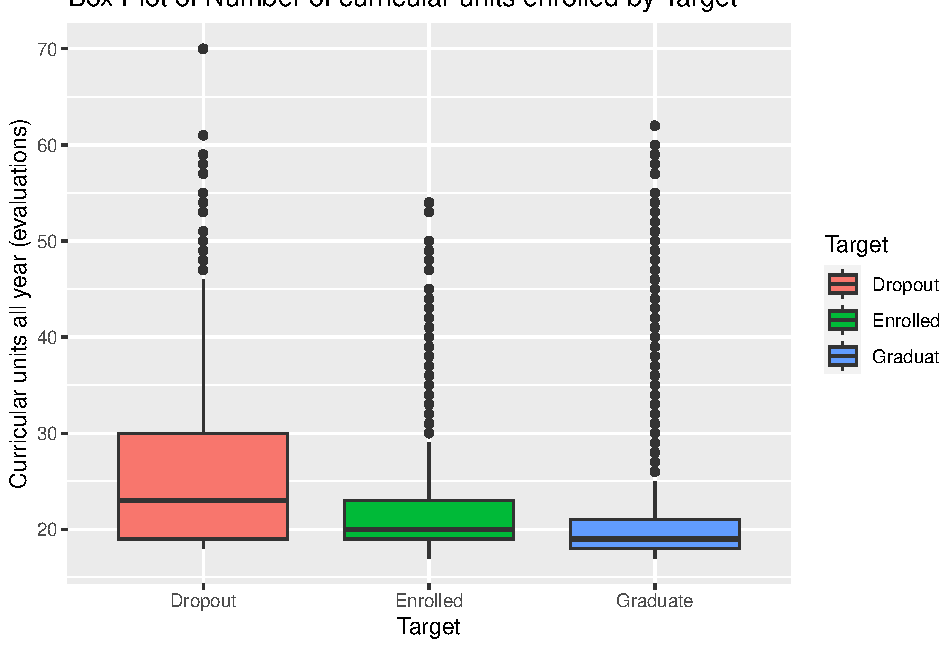
\includegraphics{exploratory_data_analysis_files/figure-latex/unnamed-chunk-20-1.pdf}

\begin{Shaded}
\begin{Highlighting}[]
\CommentTok{\# Box plot of Curricular units all year (enrolled) against \textquotesingle{}Target\textquotesingle{}}
\FunctionTok{ggplot}\NormalTok{(student\_data, }\FunctionTok{aes}\NormalTok{(}\AttributeTok{x =}\NormalTok{ Target, }\AttributeTok{y =} \StringTok{\textasciigrave{}}\AttributeTok{Curricular units all year (grade)}\StringTok{\textasciigrave{}}\NormalTok{, }\AttributeTok{fill =}\NormalTok{ Target)) }\SpecialCharTok{+} 
  \FunctionTok{geom\_boxplot}\NormalTok{() }\SpecialCharTok{+}
  \FunctionTok{labs}\NormalTok{(}\AttributeTok{title =} \StringTok{"Box Plot of Number of curricular units enrolled by Target"}\NormalTok{, }\AttributeTok{x =} \StringTok{"Target"}\NormalTok{, }\AttributeTok{y =} \StringTok{"Curricular units all year (evaluations)"}\NormalTok{)}
\end{Highlighting}
\end{Shaded}

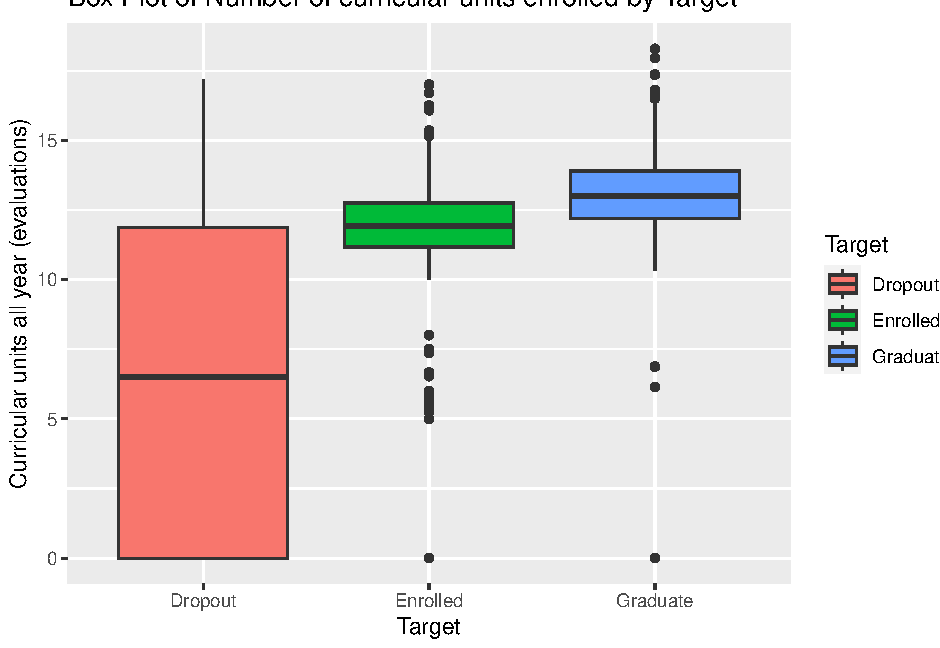
\includegraphics{exploratory_data_analysis_files/figure-latex/unnamed-chunk-21-1.pdf}

\begin{Shaded}
\begin{Highlighting}[]
\CommentTok{\# Box plot of Curricular units all year (enrolled) against \textquotesingle{}Target\textquotesingle{}}
\FunctionTok{ggplot}\NormalTok{(student\_data, }\FunctionTok{aes}\NormalTok{(}\AttributeTok{x =}\NormalTok{ Target, }\AttributeTok{y =} \StringTok{\textasciigrave{}}\AttributeTok{Curricular units all year (approved)}\StringTok{\textasciigrave{}}\NormalTok{, }\AttributeTok{fill =}\NormalTok{ Target)) }\SpecialCharTok{+} 
  \FunctionTok{geom\_boxplot}\NormalTok{() }\SpecialCharTok{+}
  \FunctionTok{labs}\NormalTok{(}\AttributeTok{title =} \StringTok{"Box Plot of Number of curricular units enrolled by Target"}\NormalTok{, }\AttributeTok{x =} \StringTok{"Target"}\NormalTok{, }\AttributeTok{y =} \StringTok{"Curricular units all year (evaluations)"}\NormalTok{)}
\end{Highlighting}
\end{Shaded}

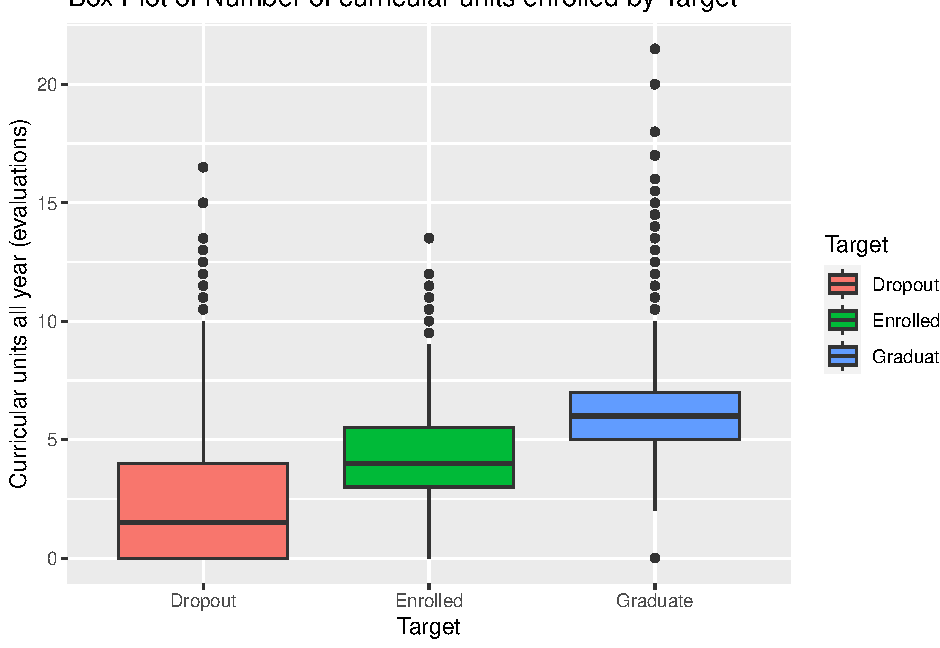
\includegraphics{exploratory_data_analysis_files/figure-latex/unnamed-chunk-22-1.pdf}
We would omit those predictors that weak association with the response
variable \texttt{Target}. After then, we select two predictors
\texttt{Curricular\ units\ all\ year\ (grade)} and
\texttt{Curricular\ units\ all\ year\ (approved)}. Also, we might want
to add some predictors that does not strongly correlate to these
predictors to add some more information about our response variable such
as \texttt{Age\ at\ enrollment}.

\textbf{Categorical Variables}

Now let's look at the data set of our categorical predictors, which we
already created and named cat\_pred. First, let's create lists of Factor
Levels, Counts, and Proportions for each of these predictors.

\begin{Shaded}
\begin{Highlighting}[]
\FunctionTok{names}\NormalTok{(cat\_pred)}
\end{Highlighting}
\end{Shaded}

\begin{verbatim}
##  [1] "Marital Status"             "Course_Enrolled"           
##  [3] "Daytime/evening attendance" "Previous qualification"    
##  [5] "Nationality"                "Mother's qualification"    
##  [7] "Father's qualification"     "Mother's occupation"       
##  [9] "Father's occupation"        "Displaced"                 
## [11] "Educational special needs"  "Debtor"                    
## [13] "Tuition fees up to date"    "Gender"                    
## [15] "Scholarship holder"         "International"
\end{verbatim}

\begin{Shaded}
\begin{Highlighting}[]
\CommentTok{\# Function }

\NormalTok{get\_factor\_summary }\OtherTok{\textless{}{-}} \ControlFlowTok{function}\NormalTok{(data, variable) \{}
  \CommentTok{\# Create a table of counts}
\NormalTok{  counts }\OtherTok{\textless{}{-}} \FunctionTok{table}\NormalTok{(data[[variable]])}
  
  \CommentTok{\# Calculate proportions}
\NormalTok{  proportions }\OtherTok{\textless{}{-}} \FunctionTok{prop.table}\NormalTok{(counts)}
  
  \CommentTok{\# Combine into a data frame}
\NormalTok{  summary\_df }\OtherTok{\textless{}{-}} \FunctionTok{data.frame}\NormalTok{(}
    \AttributeTok{Level =} \FunctionTok{names}\NormalTok{(counts),}
    \AttributeTok{Count =} \FunctionTok{as.integer}\NormalTok{(counts),}
    \AttributeTok{Proportion =}\NormalTok{ proportions}
\NormalTok{  )}
  
  \CommentTok{\# Return the summary data frame}
  \FunctionTok{return}\NormalTok{(summary\_df)}
\NormalTok{\}}

\CommentTok{\# List to store summaries}
\NormalTok{all\_summaries }\OtherTok{\textless{}{-}} \FunctionTok{list}\NormalTok{()}

\CommentTok{\# Loop through each variable in cat\_pred}
\ControlFlowTok{for}\NormalTok{ (var }\ControlFlowTok{in} \FunctionTok{names}\NormalTok{(cat\_pred)) \{}
  \CommentTok{\# Get the summary for the current variable}
\NormalTok{  summary\_df }\OtherTok{\textless{}{-}} \FunctionTok{get\_factor\_summary}\NormalTok{(cat\_pred, var)}
  
  \CommentTok{\# Store the summary in the list}
\NormalTok{  all\_summaries[[var]] }\OtherTok{\textless{}{-}}\NormalTok{ summary\_df}
  
  \CommentTok{\# Print the summary}
  \FunctionTok{cat}\NormalTok{(}\StringTok{"}\SpecialCharTok{\textbackslash{}n}\StringTok{Summary for Variable:"}\NormalTok{, var, }\StringTok{"}\SpecialCharTok{\textbackslash{}n}\StringTok{"}\NormalTok{)}
  \FunctionTok{print}\NormalTok{(summary\_df)}
\NormalTok{\}}
\end{Highlighting}
\end{Shaded}

\begin{verbatim}
## 
## Summary for Variable: Marital Status 
##     Level Count Proportion.Var1 Proportion.Freq
## 1  Single  3919          Single      0.88584991
## 2 Married   379         Married      0.08566908
## 3   Other   126           Other      0.02848101
## 
## Summary for Variable: Course_Enrolled 
##    Level Count Proportion.Var1 Proportion.Freq
## 1     33    12              33     0.002712477
## 2    171   215             171     0.048598553
## 3   8014   215            8014     0.048598553
## 4   9003   210            9003     0.047468354
## 5   9070   226            9070     0.051084991
## 6   9085   337            9085     0.076175407
## 7   9119   170            9119     0.038426763
## 8   9130   141            9130     0.031871609
## 9   9147   380            9147     0.085895118
## 10  9238   355            9238     0.080244123
## 11  9254   252            9254     0.056962025
## 12  9500   766            9500     0.173146474
## 13  9556    86            9556     0.019439421
## 14  9670   268            9670     0.060578662
## 15  9773   331            9773     0.074819168
## 16  9853   192            9853     0.043399638
## 17  9991   268            9991     0.060578662
## 
## Summary for Variable: Daytime/evening attendance 
##   Level Count Proportion.Var1 Proportion.Freq
## 1     0   483               0       0.1091772
## 2     1  3941               1       0.8908228
## 
## Summary for Variable: Previous qualification 
##                    Level Count        Proportion.Var1 Proportion.Freq
## 1    Secondary_Education  3780    Secondary_Education      0.85443038
## 2       Higher_Education   220       Higher_Education      0.04972875
## 3        Basic_Education   169        Basic_Education      0.03820072
## 4 Professional_Technical   255 Professional_Technical      0.05764014
## 
## Summary for Variable: Nationality 
##    Level Count Proportion.Var1 Proportion.Freq
## 1      1  4314               1    0.9751356239
## 2      2     2               2    0.0004520796
## 3      6    13               6    0.0029385172
## 4     11     3              11    0.0006781193
## 5     13     1              13    0.0002260398
## 6     14     1              14    0.0002260398
## 7     17     1              17    0.0002260398
## 8     21     2              21    0.0004520796
## 9     22    13              22    0.0029385172
## 10    24     5              24    0.0011301989
## 11    25     2              25    0.0004520796
## 12    26    14              26    0.0031645570
## 13    32     1              32    0.0002260398
## 14    41    38              41    0.0085895118
## 15    62     2              62    0.0004520796
## 16   100     3             100    0.0006781193
## 17   101     2             101    0.0004520796
## 18   103     3             103    0.0006781193
## 19   105     2             105    0.0004520796
## 20   108     1             108    0.0002260398
## 21   109     1             109    0.0002260398
## 
## Summary for Variable: Mother's qualification 
##                    Level Count        Proportion.Var1 Proportion.Freq
## 1    Secondary_Education  1134    Secondary_Education     0.256329114
## 2       Higher_Education   619       Higher_Education     0.139918626
## 3        Basic_Education  2526        Basic_Education     0.570976492
## 4 Professional_Technical     9 Professional_Technical     0.002034358
## 5           Unknown_None   136           Unknown_None     0.030741410
## 
## Summary for Variable: Father's qualification 
##                    Level Count        Proportion.Var1 Proportion.Freq
## 1    Secondary_Education   971    Secondary_Education     0.219633567
## 2       Higher_Education   420       Higher_Education     0.095001131
## 3        Basic_Education  2882        Basic_Education     0.651888713
## 4 Professional_Technical    24 Professional_Technical     0.005428636
## 5           Unknown_None   124           Unknown_None     0.028047953
## 
## Summary for Variable: Mother's occupation 
##                         Level Count            Proportion.Var1 Proportion.Freq
## 1                     Student   144                    Student    0.0325497288
## 2    High_Level_Professionals   430   High_Level_Professionals    0.0971971067
## 3  Intermediate_Professionals   359 Intermediate_Professionals    0.0811482821
## 4        Administrative_Staff   834       Administrative_Staff    0.1885171790
## 5             Service_Workers   563            Service_Workers    0.1272603978
## 6             Skilled_Workers   370            Skilled_Workers    0.0836347197
## 7  Operators_Assembly_Workers    36 Operators_Assembly_Workers    0.0081374322
## 8           Unskilled_Workers  1597          Unskilled_Workers    0.3609855335
## 9                Armed_Forces     4               Armed_Forces    0.0009041591
## 10              Other_Unknown    87              Other_Unknown    0.0196654611
## 
## Summary for Variable: Father's occupation 
##                         Level Count            Proportion.Var1 Proportion.Freq
## 1                     Student   128                    Student      0.02915718
## 2    High_Level_Professionals   336   High_Level_Professionals      0.07653759
## 3  Intermediate_Professionals   387 Intermediate_Professionals      0.08815490
## 4        Administrative_Staff   396       Administrative_Staff      0.09020501
## 5             Service_Workers   522            Service_Workers      0.11890661
## 6             Skilled_Workers   920            Skilled_Workers      0.20956720
## 7  Operators_Assembly_Workers   318 Operators_Assembly_Workers      0.07243736
## 8           Unskilled_Workers  1033          Unskilled_Workers      0.23530752
## 9                Armed_Forces   266               Armed_Forces      0.06059226
## 10              Other_Unknown    84              Other_Unknown      0.01913440
## 
## Summary for Variable: Displaced 
##   Level Count Proportion.Var1 Proportion.Freq
## 1     0  1998               0       0.4516275
## 2     1  2426               1       0.5483725
## 
## Summary for Variable: Educational special needs 
##   Level Count Proportion.Var1 Proportion.Freq
## 1     0  4373               0      0.98847197
## 2     1    51               1      0.01152803
## 
## Summary for Variable: Debtor 
##   Level Count Proportion.Var1 Proportion.Freq
## 1     0  3921               0        0.886302
## 2     1   503               1        0.113698
## 
## Summary for Variable: Tuition fees up to date 
##   Level Count Proportion.Var1 Proportion.Freq
## 1     0   528               0        0.119349
## 2     1  3896               1        0.880651
## 
## Summary for Variable: Gender 
##   Level Count Proportion.Var1 Proportion.Freq
## 1     0  2868               0       0.6482821
## 2     1  1556               1       0.3517179
## 
## Summary for Variable: Scholarship holder 
##   Level Count Proportion.Var1 Proportion.Freq
## 1     0  3325               0       0.7515823
## 2     1  1099               1       0.2484177
## 
## Summary for Variable: International 
##   Level Count Proportion.Var1 Proportion.Freq
## 1     0  4314               0      0.97513562
## 2     1   110               1      0.02486438
\end{verbatim}

We would want to omit or edit variables with too many or too few levels,
or those with imbalanced observations among levels. Also, using
intuition, we might keep some variables that might have an association
with students' drop out rate. Based on that, we will omit Marital Status
(Imbalance Observations between singletons and married/other), Previous
qualification (Imbalance Observations), Course\_Enrolled (too many
levels), Nationality and International (Imbalance Observations between
Portuguese and foreigners), Mother's occupation and Father's occupation
(too many levels, even after collapsing), Educational special needs
(Imbalance Observations between those with special needs and the
others).

That leaves us with these predictors:

{[}1{]} ``Daytime/evening attendance'' ``Previous qualification''\\
{[}5{]} ``Mother's qualification'' - keep ``Father's qualification'' -
keep\\
{[}9{]} ``Displaced'' ``Debtor'' - keep\\
{[}13{]} ``Tuition fees up to date'' - keep ``Gender'' ``Scholarship
holder'' - keep

\begin{Shaded}
\begin{Highlighting}[]
\FunctionTok{ggplot}\NormalTok{(student\_data, }\FunctionTok{aes}\NormalTok{(}\AttributeTok{x =} \StringTok{\textasciigrave{}}\AttributeTok{Previous qualification}\StringTok{\textasciigrave{}}\NormalTok{, }\AttributeTok{fill =}\NormalTok{ Target)) }\SpecialCharTok{+}
  \FunctionTok{geom\_bar}\NormalTok{(}\AttributeTok{position =} \StringTok{"dodge"}\NormalTok{) }\SpecialCharTok{+}
  \FunctionTok{labs}\NormalTok{(}\AttributeTok{x =} \StringTok{"Mother\textquotesingle{}s Occupation"}\NormalTok{, }\AttributeTok{y =} \StringTok{"Count"}\NormalTok{, }\AttributeTok{title =} \StringTok{"Distribution of Mother\textquotesingle{}s Occupation by Target Categories"}\NormalTok{) }\SpecialCharTok{+}
  \FunctionTok{theme\_minimal}\NormalTok{() }\SpecialCharTok{+}
  \FunctionTok{theme}\NormalTok{(}\AttributeTok{axis.text.x =} \FunctionTok{element\_text}\NormalTok{(}\AttributeTok{angle =} \DecValTok{45}\NormalTok{, }\AttributeTok{hjust =} \DecValTok{1}\NormalTok{))  }\CommentTok{\# Rotate x{-}axis labels for better readability}
\end{Highlighting}
\end{Shaded}

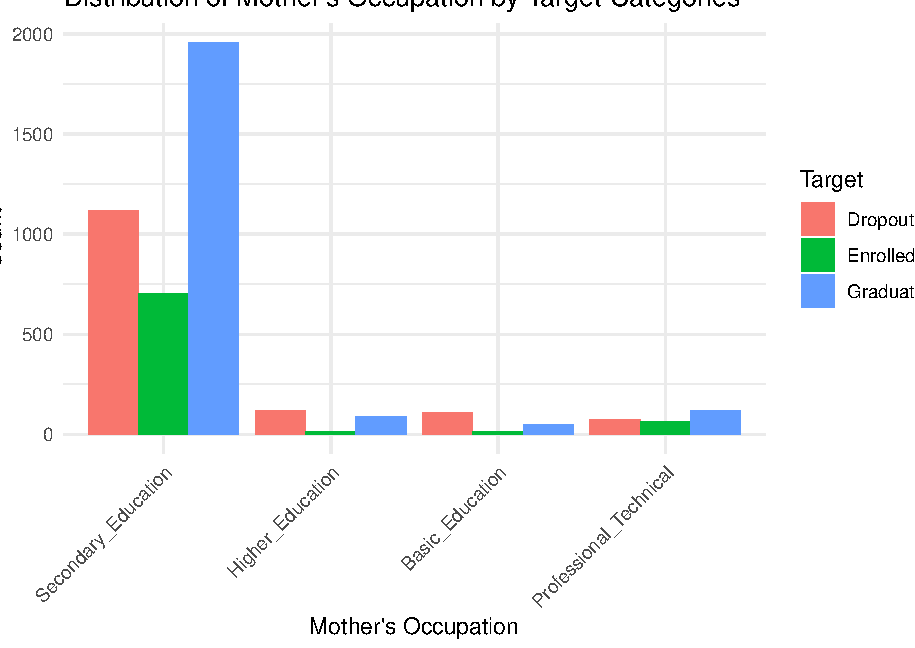
\includegraphics{exploratory_data_analysis_files/figure-latex/unnamed-chunk-25-1.pdf}

\begin{Shaded}
\begin{Highlighting}[]
\FunctionTok{ggplot}\NormalTok{(student\_data, }\FunctionTok{aes}\NormalTok{(}\AttributeTok{x =} \StringTok{\textasciigrave{}}\AttributeTok{Gender}\StringTok{\textasciigrave{}}\NormalTok{, }\AttributeTok{fill =}\NormalTok{ Target)) }\SpecialCharTok{+}
  \FunctionTok{geom\_bar}\NormalTok{(}\AttributeTok{position =} \StringTok{"dodge"}\NormalTok{) }\SpecialCharTok{+}
  \FunctionTok{labs}\NormalTok{(}\AttributeTok{x =} \StringTok{"Mother\textquotesingle{}s Occupation"}\NormalTok{, }\AttributeTok{y =} \StringTok{"Count"}\NormalTok{, }\AttributeTok{title =} \StringTok{"Distribution of Mother\textquotesingle{}s Occupation by Target Categories"}\NormalTok{) }\SpecialCharTok{+}
  \FunctionTok{theme\_minimal}\NormalTok{() }\SpecialCharTok{+}
  \FunctionTok{theme}\NormalTok{(}\AttributeTok{axis.text.x =} \FunctionTok{element\_text}\NormalTok{(}\AttributeTok{angle =} \DecValTok{45}\NormalTok{, }\AttributeTok{hjust =} \DecValTok{1}\NormalTok{))  }\CommentTok{\# Rotate x{-}axis labels for better readability}
\end{Highlighting}
\end{Shaded}

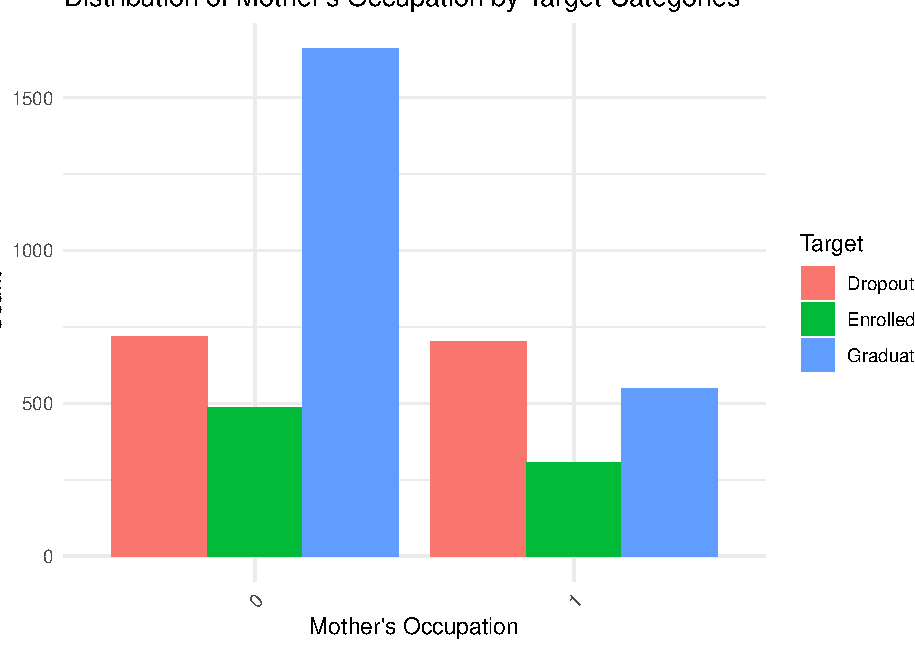
\includegraphics{exploratory_data_analysis_files/figure-latex/unnamed-chunk-26-1.pdf}

\hypertarget{analysis-for-final-report}{%
\subsection{Analysis for Final Report}\label{analysis-for-final-report}}

\begin{Shaded}
\begin{Highlighting}[]
\CommentTok{\#Remove semesterly data {-} DON\textquotesingle{}T RUN TWICE}
\NormalTok{student\_data }\OtherTok{\textless{}{-}}\NormalTok{ student\_data[,}\SpecialCharTok{{-}}\FunctionTok{c}\NormalTok{(}\DecValTok{22}\NormalTok{,}\DecValTok{23}\NormalTok{,}\DecValTok{24}\NormalTok{,}\DecValTok{25}\NormalTok{,}\DecValTok{26}\NormalTok{,}\DecValTok{27}\NormalTok{,}\DecValTok{28}\NormalTok{,}\DecValTok{29}\NormalTok{,}\DecValTok{30}\NormalTok{,}\DecValTok{31}\NormalTok{,}\DecValTok{32}\NormalTok{,}\DecValTok{33}\NormalTok{)]}
\end{Highlighting}
\end{Shaded}

\begin{Shaded}
\begin{Highlighting}[]
\NormalTok{student\_data }\OtherTok{\textless{}{-}} \FunctionTok{na.omit}\NormalTok{(student\_data)}
\NormalTok{na\_count }\OtherTok{\textless{}{-}} \FunctionTok{c}\NormalTok{()}
\ControlFlowTok{for}\NormalTok{ (i }\ControlFlowTok{in} \DecValTok{1}\SpecialCharTok{:}\DecValTok{29}\NormalTok{)\{}
\NormalTok{  na\_count[i] }\OtherTok{\textless{}{-}} \FunctionTok{sum}\NormalTok{(}\FunctionTok{is.na}\NormalTok{(student\_data[,i]))}
\NormalTok{\}}
\NormalTok{na\_count}
\end{Highlighting}
\end{Shaded}

\begin{verbatim}
##  [1] 0 0 0 0 0 0 0 0 0 0 0 0 0 0 0 0 0 0 0 0 0 0 0 0 0 0 0 0 0
\end{verbatim}

\begin{Shaded}
\begin{Highlighting}[]
\FunctionTok{names}\NormalTok{(student\_data) }\OtherTok{\textless{}{-}} \FunctionTok{make.names}\NormalTok{(}\FunctionTok{names}\NormalTok{(student\_data))}
\NormalTok{student\_data}\SpecialCharTok{$}\NormalTok{Target }\OtherTok{\textless{}{-}} \FunctionTok{factor}\NormalTok{(student\_data}\SpecialCharTok{$}\NormalTok{Target)}
\end{Highlighting}
\end{Shaded}

\begin{Shaded}
\begin{Highlighting}[]
\FunctionTok{library}\NormalTok{(rsample)}
\FunctionTok{set.seed}\NormalTok{(}\DecValTok{2024}\NormalTok{)}
\NormalTok{my\_split }\OtherTok{\textless{}{-}} \FunctionTok{initial\_split}\NormalTok{(student\_data, }\AttributeTok{prop =} \FloatTok{0.8}\NormalTok{)}
\NormalTok{train }\OtherTok{=} \FunctionTok{training}\NormalTok{(my\_split)}
\NormalTok{test }\OtherTok{=} \FunctionTok{testing}\NormalTok{(my\_split)}
\end{Highlighting}
\end{Shaded}

\hypertarget{random-forest}{%
\subsubsection{Random Forest}\label{random-forest}}

\begin{Shaded}
\begin{Highlighting}[]
\CommentTok{\#Build model}
\FunctionTok{library}\NormalTok{(randomForest)}
\end{Highlighting}
\end{Shaded}

\begin{verbatim}
## randomForest 4.7-1.1
\end{verbatim}

\begin{verbatim}
## Type rfNews() to see new features/changes/bug fixes.
\end{verbatim}

\begin{verbatim}
## 
## Attaching package: 'randomForest'
\end{verbatim}

\begin{verbatim}
## The following object is masked from 'package:ggplot2':
## 
##     margin
\end{verbatim}

\begin{verbatim}
## The following object is masked from 'package:dplyr':
## 
##     combine
\end{verbatim}

\begin{Shaded}
\begin{Highlighting}[]
\FunctionTok{set.seed}\NormalTok{(}\DecValTok{2000}\NormalTok{)}
\NormalTok{rf\_1 }\OtherTok{\textless{}{-}} \FunctionTok{randomForest}\NormalTok{(Target }\SpecialCharTok{\textasciitilde{}}\NormalTok{., train, }\AttributeTok{ntree =} \DecValTok{250}\NormalTok{, }\AttributeTok{mtry =} \DecValTok{6}\NormalTok{)}
\NormalTok{rf\_1}
\end{Highlighting}
\end{Shaded}

\begin{verbatim}
## 
## Call:
##  randomForest(formula = Target ~ ., data = train, ntree = 250,      mtry = 6) 
##                Type of random forest: classification
##                      Number of trees: 250
## No. of variables tried at each split: 6
## 
##         OOB estimate of  error rate: 22.09%
## Confusion matrix:
##          Dropout Enrolled Graduate class.error
## Dropout      851       89      185  0.24355556
## Enrolled     140      227      253  0.63387097
## Graduate      55       53     1656  0.06122449
\end{verbatim}

\begin{Shaded}
\begin{Highlighting}[]
\FunctionTok{library}\NormalTok{(yardstick)}
\end{Highlighting}
\end{Shaded}

\begin{verbatim}
## 
## Attaching package: 'yardstick'
\end{verbatim}

\begin{verbatim}
## The following object is masked from 'package:readr':
## 
##     spec
\end{verbatim}

\begin{Shaded}
\begin{Highlighting}[]
\NormalTok{rf1\_results }\OtherTok{\textless{}{-}} \FunctionTok{data.frame}\NormalTok{(}\AttributeTok{obs =}\NormalTok{ test}\SpecialCharTok{$}\NormalTok{Target,}
                         \AttributeTok{preds =} \FunctionTok{predict}\NormalTok{(rf\_1, test))}
\FunctionTok{accuracy}\NormalTok{(rf1\_results, }\AttributeTok{truth =}\NormalTok{ obs, }\AttributeTok{estimate =}\NormalTok{ preds)}
\end{Highlighting}
\end{Shaded}

\begin{verbatim}
## # A tibble: 1 x 3
##   .metric  .estimator .estimate
##   <chr>    <chr>          <dbl>
## 1 accuracy multiclass     0.769
\end{verbatim}

\begin{Shaded}
\begin{Highlighting}[]
\NormalTok{imp\_rf }\OtherTok{\textless{}{-}} \FunctionTok{as.data.frame}\NormalTok{(}\FunctionTok{importance}\NormalTok{(rf\_1))}
\NormalTok{imp\_rf}\SpecialCharTok{$}\NormalTok{names }\OtherTok{\textless{}{-}} \FunctionTok{rownames}\NormalTok{(imp\_rf)}
\FunctionTok{rownames}\NormalTok{(imp\_rf) }\OtherTok{\textless{}{-}} \ConstantTok{NULL}

\FunctionTok{ggplot}\NormalTok{(imp\_rf, }\FunctionTok{aes}\NormalTok{(}\AttributeTok{y =} \FunctionTok{reorder}\NormalTok{(names,MeanDecreaseGini), }\AttributeTok{x =}\NormalTok{ MeanDecreaseGini)) }\SpecialCharTok{+} \FunctionTok{geom\_col}\NormalTok{() }\SpecialCharTok{+} \FunctionTok{theme\_bw}\NormalTok{()}
\end{Highlighting}
\end{Shaded}

\includegraphics{exploratory_data_analysis_files/figure-latex/unnamed-chunk-33-1.pdf}

\hypertarget{boosted-trees}{%
\subsection{Boosted Trees}\label{boosted-trees}}

\begin{Shaded}
\begin{Highlighting}[]
\FunctionTok{dim}\NormalTok{(student\_data)}
\end{Highlighting}
\end{Shaded}

\begin{verbatim}
## [1] 4387   29
\end{verbatim}

\begin{Shaded}
\begin{Highlighting}[]
\FunctionTok{str}\NormalTok{(student\_data)}
\end{Highlighting}
\end{Shaded}

\begin{verbatim}
## tibble [4,387 x 29] (S3: tbl_df/tbl/data.frame)
##  $ Marital.Status                         : Factor w/ 3 levels "Single","Married",..: 1 1 1 1 2 2 1 1 1 1 ...
##  $ Application.mode                       : num [1:4387] 17 15 1 17 39 39 1 18 1 1 ...
##  $ Application.order                      : num [1:4387] 5 1 5 2 1 1 1 4 3 1 ...
##  $ Course_Enrolled                        : Factor w/ 17 levels "33","171","8014",..: 2 11 5 15 3 17 12 11 10 10 ...
##  $ Daytime.evening.attendance             : Factor w/ 2 levels "0","1": 2 2 2 2 1 1 2 2 2 2 ...
##  $ Previous.qualification                 : Factor w/ 4 levels "Secondary_Education",..: 1 1 1 1 1 3 1 1 1 1 ...
##  $ Previous.qualification..grade.         : num [1:4387] 122 160 122 122 100 ...
##  $ Nationality                            : Factor w/ 21 levels "1","2","6","11",..: 1 1 1 1 1 1 1 1 15 1 ...
##  $ Mother.s.qualification                 : Factor w/ 5 levels "Secondary_Education",..: 3 1 3 3 3 3 3 3 1 1 ...
##  $ Father.s.qualification                 : Factor w/ 5 levels "Secondary_Education",..: 1 2 3 3 3 3 3 3 1 3 ...
##  $ Mother.s.occupation                    : Factor w/ 10 levels "Student","High_Level_Professionals",..: 5 3 8 5 8 8 6 8 8 4 ...
##  $ Father.s.occupation                    : Factor w/ 10 levels "Student","High_Level_Professionals",..: 8 3 8 3 8 6 9 8 8 6 ...
##  $ Admission.grade                        : num [1:4387] 127 142 125 120 142 ...
##  $ Displaced                              : Factor w/ 2 levels "0","1": 2 2 2 2 1 1 2 2 1 2 ...
##  $ Educational.special.needs              : Factor w/ 2 levels "0","1": 1 1 1 1 1 1 1 1 1 1 ...
##  $ Debtor                                 : Factor w/ 2 levels "0","1": 1 1 1 1 1 2 1 1 1 2 ...
##  $ Tuition.fees.up.to.date                : Factor w/ 2 levels "0","1": 2 1 1 2 2 2 2 1 2 1 ...
##  $ Gender                                 : Factor w/ 2 levels "0","1": 2 2 2 1 1 2 1 2 1 1 ...
##  $ Scholarship.holder                     : Factor w/ 2 levels "0","1": 1 1 1 1 1 1 2 1 2 1 ...
##  $ Age.at.enrollment                      : num [1:4387] 20 19 19 20 45 50 18 22 21 18 ...
##  $ International                          : Factor w/ 2 levels "0","1": 1 1 1 1 1 1 1 1 2 1 ...
##  $ Unemployment.rate                      : num [1:4387] 10.8 13.9 10.8 9.4 13.9 16.2 15.5 15.5 16.2 8.9 ...
##  $ Inflation.rate                         : num [1:4387] 1.4 -0.3 1.4 -0.8 -0.3 0.3 2.8 2.8 0.3 1.4 ...
##  $ GDP                                    : num [1:4387] 1.74 0.79 1.74 -3.12 0.79 -0.92 -4.06 -4.06 -0.92 3.51 ...
##  $ Target                                 : Factor w/ 3 levels "Dropout","Enrolled",..: 1 3 1 3 3 3 3 1 3 1 ...
##  $ Curricular.units.all.year..enrolled.   : num [1:4387] 0 6 6 6 6 5 7.5 5 6 6 ...
##  $ Curricular.units.all.year..evaluations.: num [1:4387] 0 6 0 9 7.5 13.5 8.5 5 7.5 11.5 ...
##  $ Curricular.units.all.year..approved.   : num [1:4387] 0 6 0 5.5 5.5 5 7.5 0 6 3.5 ...
##  $ Curricular.units.all.year..grade.      : num [1:4387] 0 13.8 0 12.9 12.7 ...
##  - attr(*, "na.action")= 'omit' Named int [1:37] 32 200 369 506 611 927 929 997 1088 1204 ...
##   ..- attr(*, "names")= chr [1:37] "32" "200" "369" "506" ...
\end{verbatim}

Currently we have 29 variables. \texttt{XGBoost} only accepts numerical
variables, while most of our predictors are categorical. We will
deselect the variables with too many factors and/or minimal importance.

\begin{Shaded}
\begin{Highlighting}[]
\NormalTok{boosted\_student\_data }\OtherTok{\textless{}{-}}\NormalTok{ student\_data[, }\SpecialCharTok{{-}}\FunctionTok{c}\NormalTok{(}\DecValTok{1}\NormalTok{,}\DecValTok{2}\NormalTok{,}\DecValTok{5}\NormalTok{,}\DecValTok{6}\NormalTok{,}\DecValTok{8}\NormalTok{,}\DecValTok{9}\NormalTok{,}\DecValTok{10}\NormalTok{,}\DecValTok{14}\NormalTok{,}\DecValTok{15}\NormalTok{,}\DecValTok{21}\NormalTok{)]}
\FunctionTok{str}\NormalTok{(boosted\_student\_data)}
\end{Highlighting}
\end{Shaded}

\begin{verbatim}
## tibble [4,387 x 19] (S3: tbl_df/tbl/data.frame)
##  $ Application.order                      : num [1:4387] 5 1 5 2 1 1 1 4 3 1 ...
##  $ Course_Enrolled                        : Factor w/ 17 levels "33","171","8014",..: 2 11 5 15 3 17 12 11 10 10 ...
##  $ Previous.qualification..grade.         : num [1:4387] 122 160 122 122 100 ...
##  $ Mother.s.occupation                    : Factor w/ 10 levels "Student","High_Level_Professionals",..: 5 3 8 5 8 8 6 8 8 4 ...
##  $ Father.s.occupation                    : Factor w/ 10 levels "Student","High_Level_Professionals",..: 8 3 8 3 8 6 9 8 8 6 ...
##  $ Admission.grade                        : num [1:4387] 127 142 125 120 142 ...
##  $ Debtor                                 : Factor w/ 2 levels "0","1": 1 1 1 1 1 2 1 1 1 2 ...
##  $ Tuition.fees.up.to.date                : Factor w/ 2 levels "0","1": 2 1 1 2 2 2 2 1 2 1 ...
##  $ Gender                                 : Factor w/ 2 levels "0","1": 2 2 2 1 1 2 1 2 1 1 ...
##  $ Scholarship.holder                     : Factor w/ 2 levels "0","1": 1 1 1 1 1 1 2 1 2 1 ...
##  $ Age.at.enrollment                      : num [1:4387] 20 19 19 20 45 50 18 22 21 18 ...
##  $ Unemployment.rate                      : num [1:4387] 10.8 13.9 10.8 9.4 13.9 16.2 15.5 15.5 16.2 8.9 ...
##  $ Inflation.rate                         : num [1:4387] 1.4 -0.3 1.4 -0.8 -0.3 0.3 2.8 2.8 0.3 1.4 ...
##  $ GDP                                    : num [1:4387] 1.74 0.79 1.74 -3.12 0.79 -0.92 -4.06 -4.06 -0.92 3.51 ...
##  $ Target                                 : Factor w/ 3 levels "Dropout","Enrolled",..: 1 3 1 3 3 3 3 1 3 1 ...
##  $ Curricular.units.all.year..enrolled.   : num [1:4387] 0 6 6 6 6 5 7.5 5 6 6 ...
##  $ Curricular.units.all.year..evaluations.: num [1:4387] 0 6 0 9 7.5 13.5 8.5 5 7.5 11.5 ...
##  $ Curricular.units.all.year..approved.   : num [1:4387] 0 6 0 5.5 5.5 5 7.5 0 6 3.5 ...
##  $ Curricular.units.all.year..grade.      : num [1:4387] 0 13.8 0 12.9 12.7 ...
##  - attr(*, "na.action")= 'omit' Named int [1:37] 32 200 369 506 611 927 929 997 1088 1204 ...
##   ..- attr(*, "names")= chr [1:37] "32" "200" "369" "506" ...
\end{verbatim}

\begin{Shaded}
\begin{Highlighting}[]
\NormalTok{boosted\_student\_data}\SpecialCharTok{$}\NormalTok{Debtor }\OtherTok{\textless{}{-}} \FunctionTok{as.numeric}\NormalTok{(}\FunctionTok{as.character}\NormalTok{(boosted\_student\_data}\SpecialCharTok{$}\NormalTok{Debtor))}
\NormalTok{boosted\_student\_data}\SpecialCharTok{$}\NormalTok{Tuition.fees.up.to.date }\OtherTok{\textless{}{-}} \FunctionTok{as.numeric}\NormalTok{(}\FunctionTok{as.character}\NormalTok{(boosted\_student\_data}\SpecialCharTok{$}\NormalTok{Tuition.fees.up.to.date))}
\NormalTok{boosted\_student\_data}\SpecialCharTok{$}\NormalTok{Gender }\OtherTok{\textless{}{-}} \FunctionTok{as.numeric}\NormalTok{(}\FunctionTok{as.character}\NormalTok{(boosted\_student\_data}\SpecialCharTok{$}\NormalTok{Gender))}
\NormalTok{boosted\_student\_data}\SpecialCharTok{$}\NormalTok{Scholarship.holder }\OtherTok{\textless{}{-}} \FunctionTok{as.numeric}\NormalTok{(}\FunctionTok{as.character}\NormalTok{(boosted\_student\_data}\SpecialCharTok{$}\NormalTok{Scholarship.holder))}
\end{Highlighting}
\end{Shaded}

\begin{Shaded}
\begin{Highlighting}[]
\FunctionTok{str}\NormalTok{(boosted\_student\_data)}
\end{Highlighting}
\end{Shaded}

\begin{verbatim}
## tibble [4,387 x 19] (S3: tbl_df/tbl/data.frame)
##  $ Application.order                      : num [1:4387] 5 1 5 2 1 1 1 4 3 1 ...
##  $ Course_Enrolled                        : Factor w/ 17 levels "33","171","8014",..: 2 11 5 15 3 17 12 11 10 10 ...
##  $ Previous.qualification..grade.         : num [1:4387] 122 160 122 122 100 ...
##  $ Mother.s.occupation                    : Factor w/ 10 levels "Student","High_Level_Professionals",..: 5 3 8 5 8 8 6 8 8 4 ...
##  $ Father.s.occupation                    : Factor w/ 10 levels "Student","High_Level_Professionals",..: 8 3 8 3 8 6 9 8 8 6 ...
##  $ Admission.grade                        : num [1:4387] 127 142 125 120 142 ...
##  $ Debtor                                 : num [1:4387] 0 0 0 0 0 1 0 0 0 1 ...
##  $ Tuition.fees.up.to.date                : num [1:4387] 1 0 0 1 1 1 1 0 1 0 ...
##  $ Gender                                 : num [1:4387] 1 1 1 0 0 1 0 1 0 0 ...
##  $ Scholarship.holder                     : num [1:4387] 0 0 0 0 0 0 1 0 1 0 ...
##  $ Age.at.enrollment                      : num [1:4387] 20 19 19 20 45 50 18 22 21 18 ...
##  $ Unemployment.rate                      : num [1:4387] 10.8 13.9 10.8 9.4 13.9 16.2 15.5 15.5 16.2 8.9 ...
##  $ Inflation.rate                         : num [1:4387] 1.4 -0.3 1.4 -0.8 -0.3 0.3 2.8 2.8 0.3 1.4 ...
##  $ GDP                                    : num [1:4387] 1.74 0.79 1.74 -3.12 0.79 -0.92 -4.06 -4.06 -0.92 3.51 ...
##  $ Target                                 : Factor w/ 3 levels "Dropout","Enrolled",..: 1 3 1 3 3 3 3 1 3 1 ...
##  $ Curricular.units.all.year..enrolled.   : num [1:4387] 0 6 6 6 6 5 7.5 5 6 6 ...
##  $ Curricular.units.all.year..evaluations.: num [1:4387] 0 6 0 9 7.5 13.5 8.5 5 7.5 11.5 ...
##  $ Curricular.units.all.year..approved.   : num [1:4387] 0 6 0 5.5 5.5 5 7.5 0 6 3.5 ...
##  $ Curricular.units.all.year..grade.      : num [1:4387] 0 13.8 0 12.9 12.7 ...
##  - attr(*, "na.action")= 'omit' Named int [1:37] 32 200 369 506 611 927 929 997 1088 1204 ...
##   ..- attr(*, "names")= chr [1:37] "32" "200" "369" "506" ...
\end{verbatim}

\begin{Shaded}
\begin{Highlighting}[]
\FunctionTok{library}\NormalTok{(Matrix)}
\NormalTok{sparse\_matrix }\OtherTok{\textless{}{-}} \FunctionTok{sparse.model.matrix}\NormalTok{(Target }\SpecialCharTok{\textasciitilde{}}\NormalTok{., }\AttributeTok{data =}\NormalTok{ boosted\_student\_data)[,}\SpecialCharTok{{-}}\DecValTok{1}\NormalTok{]}
\FunctionTok{colnames}\NormalTok{(sparse\_matrix)}
\end{Highlighting}
\end{Shaded}

\begin{verbatim}
##  [1] "Application.order"                            
##  [2] "Course_Enrolled171"                           
##  [3] "Course_Enrolled8014"                          
##  [4] "Course_Enrolled9003"                          
##  [5] "Course_Enrolled9070"                          
##  [6] "Course_Enrolled9085"                          
##  [7] "Course_Enrolled9119"                          
##  [8] "Course_Enrolled9130"                          
##  [9] "Course_Enrolled9147"                          
## [10] "Course_Enrolled9238"                          
## [11] "Course_Enrolled9254"                          
## [12] "Course_Enrolled9500"                          
## [13] "Course_Enrolled9556"                          
## [14] "Course_Enrolled9670"                          
## [15] "Course_Enrolled9773"                          
## [16] "Course_Enrolled9853"                          
## [17] "Course_Enrolled9991"                          
## [18] "Previous.qualification..grade."               
## [19] "Mother.s.occupationHigh_Level_Professionals"  
## [20] "Mother.s.occupationIntermediate_Professionals"
## [21] "Mother.s.occupationAdministrative_Staff"      
## [22] "Mother.s.occupationService_Workers"           
## [23] "Mother.s.occupationSkilled_Workers"           
## [24] "Mother.s.occupationOperators_Assembly_Workers"
## [25] "Mother.s.occupationUnskilled_Workers"         
## [26] "Mother.s.occupationArmed_Forces"              
## [27] "Mother.s.occupationOther_Unknown"             
## [28] "Father.s.occupationHigh_Level_Professionals"  
## [29] "Father.s.occupationIntermediate_Professionals"
## [30] "Father.s.occupationAdministrative_Staff"      
## [31] "Father.s.occupationService_Workers"           
## [32] "Father.s.occupationSkilled_Workers"           
## [33] "Father.s.occupationOperators_Assembly_Workers"
## [34] "Father.s.occupationUnskilled_Workers"         
## [35] "Father.s.occupationArmed_Forces"              
## [36] "Father.s.occupationOther_Unknown"             
## [37] "Admission.grade"                              
## [38] "Debtor"                                       
## [39] "Tuition.fees.up.to.date"                      
## [40] "Gender"                                       
## [41] "Scholarship.holder"                           
## [42] "Age.at.enrollment"                            
## [43] "Unemployment.rate"                            
## [44] "Inflation.rate"                               
## [45] "GDP"                                          
## [46] "Curricular.units.all.year..enrolled."         
## [47] "Curricular.units.all.year..evaluations."      
## [48] "Curricular.units.all.year..approved."         
## [49] "Curricular.units.all.year..grade."
\end{verbatim}

\begin{Shaded}
\begin{Highlighting}[]
\FunctionTok{require}\NormalTok{(xgboost)}
\end{Highlighting}
\end{Shaded}

\begin{verbatim}
## Loading required package: xgboost
\end{verbatim}

\begin{verbatim}
## 
## Attaching package: 'xgboost'
\end{verbatim}

\begin{verbatim}
## The following object is masked from 'package:dplyr':
## 
##     slice
\end{verbatim}

\begin{Shaded}
\begin{Highlighting}[]
\CommentTok{\#library(caret)}
\CommentTok{\#set.seed(2024)}
\CommentTok{\#boostedIndex \textless{}{-} createDataPartition(sparse\_matrix$Target, p=.8, list = FALSE, times = 1)}
\CommentTok{\#boosted\_train \textless{}{-} sparse\_matrix[boostedIndex,]}
\CommentTok{\#boosted\_test \textless{}{-} sparse\_matrix[{-}boostedIndex,]}
\end{Highlighting}
\end{Shaded}


\end{document}
